% #############################################################################
% This is the MAIN DOCUMENT of the Thesis MSc TEMPLATE.
% The content for the Thesis MSc is to be written in separate documents
% located in the folder ./Chapters
%         Aknowledgments.tex
%         Abstract.tex
%         KeyWords.tex
%         Resumo.tex
%         PalavrasChave.tex
%         Acronyms.tex
%         Front_Cover.tex
%         Chapter_1.tex ....Chapter_2 .....
%         ApendixA.tex ... ApendixB.tex...
% -----------------------------------------------------------------------------
% The class "istulthesis" is based on the standard LaTeX 'report' class.
% It can be used for Instituto Superior Tecnico thesis, as it follows the 
% regulations published by the Scientific Council of IST.
% The class defines the document style. 
% IST requires the thesis to be written in Arial or similar. 
% Two arguments in '\documentclass' allow you to define the thesis font: 
% 'Helvetica' and 'AvantGarde', which transforms 
% the default LaTeX font into Helvetica or AvantGarde, respectively.
% #############################################################################
% The document is automatically set for english or portuguese by just selecting
% the MAIN LANGUAGE in file 'Thesis-MSc-Preamble_commands.tex' 
% #############################################################################
% Thesis-MSc
% Version 2.0, August 2018
% BY: Rui Santos Cruz, rui.s.cruz@tecnico.ulisboa.pt
% #############################################################################
% !TEX root = ./main.tex
% -----------------------------------------------------------------------------
%
\documentclass[defaultstyle,10pt,Helvetica]{istulthesis}
%
% -----------------------------------------------------------------------------
% The Preamble document contains all the necessary Packages for typesetting
% Modify it to suit your needs
% -----------------------------------------------------------------------------
% #############################################################################
% Preamble for Thesis-MSc in English or Portuguese
% Required Packages and commands
% --> Please Choose the MAIN LANGUAGE for the Thesis in package BABEL (below)
% !TEX root = ./main.tex
% #############################################################################
% Thesis-MSc
% Version 2.0, August 2018
% BY: Rui Santos Cruz, rui.s.cruz@tecnico.ulisboa.pt
% #############################################################################
%
% -----------------------------------------------------------------------------
% PACKAGES ucs, utf8x, babel, iflang:
% -----------------------------------------------------------------------------
% The 'ucs' package provides support for using UTF-8 in LaTeX documents. 
% However in most situations it is not required.
\usepackage{ucs}
% The 'utf8x' package contains support for using UTF-8 as input encoding. 
\usepackage[utf8x]{inputenc}
% The 'babel' package may correct some hyphenation issues of LaTeX. 
% Select your MAIN LANGUAGE for the Thesis with the 'main=' option.
\usepackage[main=english,portuguese]{babel}
% The 'iflang' package is used to help determine the language being used. 
\usepackage{iflang}

% -----------------------------------------------------------------------------
% PACKAGE scrbase:
% -----------------------------------------------------------------------------
% The 'scrbase' package is used to help redefining document structure.
\usepackage{scrbase}
% -----------------------------------------------------------------------------
% PACKAGE mathtools, amsmath, amsthm, amssymb, amsfonts, nicefrac:
% -----------------------------------------------------------------------------
% These packages are typically required. 
% Among many other things they add the possibility to put symbols in bold
% by using \boldsymbol (not \mathbf); defines additional fonts and symbols;
% adds the \eqref command for citing equations.
\usepackage{mathtools, amsmath, amsthm, amssymb, amsfonts}
\usepackage{nicefrac}
%
% -----------------------------------------------------------------------------
% PACKAGE tikz:
% -----------------------------------------------------------------------------
% Tikz  for creating graphics programmatically.
\usepackage{tikz}
\usetikzlibrary{shapes.geometric, arrows, positioning}
% -----------------------------------------------------------------------------
% PACKAGES array, booktabs, multirow, colortbl, ctable, spreadtab:
% -----------------------------------------------------------------------------
% These packages are most usefull for advanced tables. 
% 'multirow' allows to join rows throuhg the command \multirow which works
% similarly with the command \multicolumn.
% The 'colortbl' package allows to color the table (foreground and background)
% The 'ctable' package provides commands to easily typeset centered or left or
% right aligned tables.
% The package 'booktabs' provide some additional commands to enhance
% the quality of tables
% The 'longtable' package is only required when tables extend beyond the length
% of one page, which typically does not happen and should be avoided
\usepackage{array}
\usepackage{booktabs}
\usepackage{multirow}
\usepackage{colortbl}
\usepackage{ctable}
\usepackage{spreadtab}
\usepackage{longtable}
%
% -----------------------------------------------------------------------------
% PACKAGES graphicx, subfigure:
% -----------------------------------------------------------------------------
% The package 'graphicx' supports formats PNG and JPG.
% Package 'subfigure' allows to place figures within figures with own caption. 
% For each of the subfigures use the command \subfigure.
\usepackage{graphicx}
\usepackage[hang,small,bf,tight]{subfigure}
%
% -----------------------------------------------------------------------------
% PACKAGE caption:
% -----------------------------------------------------------------------------
% The 'caption' package offers customization of captions in floating 
% environments such figure and table
% \usepackage[hang,small,bf]{caption}
\usepackage[format=hang,labelfont=bf,font=small]{caption} 
% the following customization adds vertical space between caption and the table
\captionsetup[table]{skip=10pt}
%
% -----------------------------------------------------------------------------
% PACKAGE algorithmic, algorithm, algorithm2e:
% -----------------------------------------------------------------------------
% These packages are required if you need to describe an algorithm.
% The preference is for using 'algorithm2e'
%\usepackage{algorithmic}
%\usepackage[chapter]{algorithm}
\usepackage[ruled,vlined,algochapter,norelsize,\languagename]{algorithm2e}
%
% -----------------------------------------------------------------------------
% PACKAGE listings
% -----------------------------------------------------------------------------
% These packages are required if you need to list code snippets.
\usepackage{listings}
% Nicely syntax highlighted m-code in LaTeX documents with stylefile mcode.sty
% http://www.mathworks.com/matlabcentral/fileexchange/8015-m-code-latex-package
\usepackage[numbered]{./tables_and_code/mcode}
%
% -----------------------------------------------------------------------------
% Re-define listings captions and titles based on language.
\newcaptionname{portuguese}{\lstlistingname}{Listagem} % Listings CAPTIONS
\newcaptionname{portuguese}{\lstlistlistingname}{Listagens} % LIST of LISTINGS
%
% -----------------------------------------------------------------------------
% PACKAGE csquotes
% -----------------------------------------------------------------------------
% Quotation helper package
\usepackage{csquotes}
%
% -----------------------------------------------------------------------------
% PACKAGE todonotes
% -----------------------------------------------------------------------------
% Create TODO Notes in text
% The notes can be made invisible by just using the 'disable' option:
%\usepackage[textwidth=2cm, textsize=small]{todonotes}
\usepackage[textwidth=2cm, textsize=small, disable]{todonotes}
\setlength{\marginparwidth}{2cm}
%
% -----------------------------------------------------------------------------
% PACKAGE changes
% -----------------------------------------------------------------------------
% Track changes in document (changes in pdf preview).
%% Use "final" option to make all tracking markups invisible.
\usepackage[authormarkup=superscript,authormarkuptext=id,markup=underlined,ulem={ULforem,normalbf},final]{changes}
%\usepackage[authormarkup=superscript,authormarkuptext=id,markup=underlined,ulem={ULforem,normalbf}]{changes}
% commands:
% \added[id=xx]{text}
% \deleted[id=xx]{text}
% \replaced[id=xx]{deleted text}{added text}
% -----------------------------------------------------------------------------
% PACKAGES xcolor, color
% -----------------------------------------------------------------------------
% These packages are required for list code snippets.
\usepackage{xcolor}
\usepackage{color}
% The following special color definitions are used in the IST Thesis
\definecolor{forestgreen}{RGB}{34,139,34}
\definecolor{orangered}{RGB}{239,134,64}
\definecolor{lightred}{rgb}{1,0.4,0.5}
\definecolor{orange}{rgb}{1,0.45,0.13}	
\definecolor{darkblue}{rgb}{0.0,0.0,0.6}
\definecolor{lightblue}{rgb}{0.1,0.57,0.7}
\definecolor{gray}{rgb}{0.4,0.4,0.4}
\definecolor{lightgray}{rgb}{0.95, 0.95, 0.95}
\definecolor{darkgray}{rgb}{0.4, 0.4, 0.4}
\definecolor{editorGray}{rgb}{0.95, 0.95, 0.95}
\definecolor{editorOcher}{rgb}{1, 0.5, 0} % #FF7F00 -> rgb(239, 169, 0)
\definecolor{chaptergrey}{rgb}{0.6,0.6,0.6}
\definecolor{editorGreen}{rgb}{0, 0.5, 0} % #007C00 -> rgb(0, 124, 0)
\definecolor{olive}{rgb}{0.17,0.59,0.20}
\definecolor{brown}{rgb}{0.69,0.31,0.31}
\definecolor{purple}{rgb}{0.38,0.18,0.81}
%
% -----------------------------------------------------------------------------
% PACKAGE setspace:
% ----------------------------------------------------------------------------
% Provides support for setting the spacing between lines in a document. 
% Package options include single spacing, one half spacing, and double spacing. 
% Alternatively the spacing can be changed as required with:
% \singlespacing, \onehalfspacing, and \doublespacing commands
\usepackage{setspace}
%
% -----------------------------------------------------------------------------
% PACKAGE paralist
% -----------------------------------------------------------------------------
% This package provides the 'inparaenum' environment for inline lists
\usepackage{paralist}
% usage:
% \begin{inparaenum}[(a)]
% \item bla
% \item bla, bla
% \end{inparaenum}
% -----------------------------------------------------------------------------
% PACKAGE cite:
% -----------------------------------------------------------------------------
% The 'cite' package will result in citation numbers being automatically
% sorted and properly "ranged". i.e.,
% [1], [2], [5]--[7], [9]
\usepackage{cite}
%
% -----------------------------------------------------------------------------
% PACKAGE acronym:
% -----------------------------------------------------------------------------
% The package 'acronym' garantees that all acronyms definitions are 
% given at the first usage. 
% IMPORTANT: do not use acronyms in titles/captions; otherwise the definition 
% will appear on the table of contents.
\usepackage[printonlyused]{acronym}
%
% -----------------------------------------------------------------------------
% PACKAGE hyperref
% -----------------------------------------------------------------------------
% Set links for references and citations in document
\usepackage{hyperref}
% pre-configuration of hyperref
\hypersetup{ colorlinks=true,
             citecolor=cyan,
             linkcolor=darkgray,
             urlcolor=teal,
             breaklinks=true,
             bookmarksnumbered=true,
             bookmarksopen=true,
             pdftitle=\@title, % THESIS TITLE
             pdfauthor=\@author,  % YOUR NAME
             pdfcreator=\@author,   % YOUR NAME
}
%
% -----------------------------------------------------------------------------
% PACKAGE url:
% -----------------------------------------------------------------------------
% Provides better support for handling and breaking URLs.
\usepackage{url} 
%
% -----------------------------------------------------------------------------
% PACKAGE Cleveref:
% -----------------------------------------------------------------------------
% Clever Referencing of document parts
% Note: portuguese is supported through "brazilian" option
\usepackage[\IfLanguageName{english}{english}{brazilian}]{cleveref}
%
% -----------------------------------------------------------------------------
% PACKAGE enumitem:
% -----------------------------------------------------------------------------
%For enhanced enumeration of lists
%\usepackage{enumitem}
\usepackage[shortlabels]{enumitem}
\setlist[description]{leftmargin=\parindent,labelindent=\parindent,itemsep=1pt,parsep=0pt,topsep=0pt}
%
% #############################################################################
% GLOBAL FORMATTING OF THE THESIS DOCUMENT before using FANCY stuff
% Set paragraph counter to alphanumeric mode
\renewcommand{\theparagraph}{\Alph{paragraph}~--}
\hoffset 0in
\voffset 0in
\oddsidemargin 0 cm
\evensidemargin 0 cm
\marginparsep 0in
\topmargin -0.25cm
\textwidth 16 cm
\textheight 22.4 cm
\makeatletter
% package indentfirst says \let\@afterindentfalse\@afterindenttrue
% and we revert this modification, reinstating the original definitio
% of \@afterindentfalse
\def\@afterindentfalse{\let\if@afterindent\iffalse}
\makeatother
% -----------------------------------------------------------------------------
% PACKAGE fancyhdr:
% -----------------------------------------------------------------------------
% The fancyhdr macro package allows to customize page headers and footers.
\usepackage{fancyhdr}
\pagestyle{fancy}
\renewcommand{\chaptermark}[1]{\markboth{\thechapter.\ #1}{}}
\renewcommand{\sectionmark}[1]{\markright{\thesection\ #1}}
\fancyhead{}
\renewcommand{\headrulewidth}{0.0pt}
\renewcommand{\footrulewidth}{0.0pt}
\addtolength{\headheight}{2pt} % make space for the rule
\fancypagestyle{plain}{%
   \fancyhead{} % get rid of headers
   \renewcommand{\headrulewidth}{0pt} % and the line
   \renewcommand{\footrulewidth}{0pt}
}
\fancypagestyle{blank}{%
   \fancyhf{} % get rid of headers and footers
   \renewcommand{\headrulewidth}{0pt} % and the line
   \renewcommand{\footrulewidth}{0pt}
}
\fancypagestyle{abstract}{%
   \fancyhead{}
   \renewcommand{\headrulewidth}{0pt}
   \renewcommand{\footrulewidth}{0.0pt}
}
\fancypagestyle{document}{%
	\fancyhead{}
	\renewcommand{\headrulewidth}{0.5pt}
	\renewcommand{\footrulewidth}{0.5pt}
	\addtolength{\headheight}{2pt} % make space for the rule
}
\setcounter{secnumdepth} {5}
\setcounter{tocdepth} {5}
\renewcommand{\thesubsubsection}{\thesubsection.\Alph{subsubsection}}
\renewcommand{\subfigtopskip}{0.3 cm}
\renewcommand{\subfigbottomskip}{0.2 cm}
\renewcommand{\subfigcapskip}{0.3 cm}
\renewcommand{\subfigcapmargin}{0.2 cm}
%
% -----------------------------------------------------------------------------
% PACKAGE minitoc:
% -----------------------------------------------------------------------------
% Package 'minitoc' creates a mini-table of contents (a “minitoc”) at 
% the beginning of each chapter of a document.
% This packages are required for the \fancychapter configuration
\usepackage{minitoc}
\setcounter{minitocdepth}{1}
\setlength{\mtcindent}{24pt}
\renewcommand{\mtcfont}{\small\rm}
\renewcommand{\mtcSfont}{\small\bf}
\renewcommand*{\kernafterminitoc}{\kern0.\baselineskip\kern0.ex}
\mtcselectlanguage{\languagename} 
% Now prepare the MINITOC
\def\boxedverbatim{%
  \def\verbatim@processline{%
    {\setbox0=\hbox{\the\verbatim@line}%
    \hsize=\wd0 \the\verbatim@line\par}}%
  \@minipagetrue%%%DPC%%%
  \@tempswatrue%%%DPC%%%
  \setbox0=\vbox\bgroup\vspace*{0.2cm}\footnotesize\verbatim
}
\def\endboxedverbatim{%
  \endverbatim
  \unskip\setbox0=\lastbox %%%DPC%%%
  \hspace*{0.2cm}
  \vspace*{-0.2cm}
  \egroup
  \fbox{\box0}% <<<=== change here for centering,...
}
% Now prepare the CHAPTER Number
\newcommand*{\chapnumfont}{%
%   \usefont{T1}{\@defaultcnfont}{b}{n}\fontsize{100}{130}\selectfont%
  \usefont{T1}{pbk}{b}{n}
  \fontsize{150}{130}
  \selectfont
  \color{chaptergrey}
}
\makeatletter
\def\@makechapterhead#1{%
  \vspace*{50\p@}%
  {\parindent \z@ \raggedright \normalfont
    {\chapnumfont\ifnum \c@secnumdepth >\m@ne
%         \huge\bfseries \@chapapp\space \thechapter
        \raggedleft\bfseries \thechapter
        \par\nobreak
        \vskip 20\p@
    \fi}
    \interlinepenalty\@M
    {\raggedleft\Huge \bfseries #1\par\nobreak}
    \vskip 40\p@
  }}
\makeatother
% Now put it all together as a command \fancychapter
\newcommand{\fancychapter}[1]{\chapter{#1}\vfill\minitoc\pagebreak}
%
% #############################################################################
% ADDITIONAL COMMANDS AND CONFIGURATIONS
% #############################################################################
% This commmand allows to place horizontal lines with a custom width... 
% replaces the standard hline command
\newcommand{\hlinew}[1]{%
  \noalign{\ifnum0=`}\fi\hrule \@height #1 \futurelet
   \reserved@a\@xhline}
%   
% -----------------------------------------------------------------------------
% This command defines some marks... USEFUL FOR TABLES.
\def\Mark#1{\raisebox{0pt}[0pt][0pt]{\textsuperscript{\footnotesize\ensuremath{\ifcase#1\or *\or \dagger\or \ddagger\or%
    \mathsection\or \mathparagraph\or \|\or **\or \dagger\dagger%
    \or \ddagger\ddagger \else\textsuperscript{\expandafter\romannumeral#1}\fi}}}}
%
% -----------------------------------------------------------------------------
% The following configurations are used for LISTINGS of certain languages
\lstdefinestyle{XML} {
	language=XML,
	extendedchars=true, 
	breaklines=true,
	breakatwhitespace=true,
	emph={},
	emphstyle=\color{red},
	basicstyle=\small,
	xleftmargin=17pt,
	columns=fullflexible,
	commentstyle=\color{gray}\upshape,
	morestring=[b][\color{brown}]",
	morecomment=[s]{<?}{?>},
	morecomment=[s][\color{forestgreen}]{<!--}{-->},
	keywordstyle=\color{orangered},
	stringstyle=\ttfamily\color{black},
	% stringstyle=\ttfamily\color{black}\normalfont,
	tagstyle=\color{blue},
	% tagstyle=\color{darkblue}\bf,
	morekeywords={asn,action,addrType,abilityNAT,audioSampleRate,audiChannels,,bandwidth,bitmapSize,bitRate,connection,codecs,concurrentLinks,dependency,duration,frameRate,from,height,ip,id,lang,mimeType,onlineTime,peerMode,port,priority,peerProtocol,property,release,to,tier,type,transactionID,url,uploadBWlevel,version,width},
	otherkeywords={attribute,xmlns,schemaLocation,PresentationType,availabilityStartTime,availabilityEndTime,minimumUpdatePeriod,minBufferTime,UpdateTime},
}
% ----------------------------------------------------------------------------
\lstdefinelanguage{Assembler}{
	morecomment=[l];,
	keywords={ADD,ADDC,SUB,SUBB,CMP,MUL,DIV,MOD,NEG,AND,OR,NOT,XOR,TEST,BIT,SET,EI,EI0,EI1,EI2,EI3,SETC,EDMA,CLR,DI,DI0,DI1,DI2,DI3,CLRC,SHR,SHL,SHRA,SHLA,ROR,ROL,RORC,ROLC,MOV,MOVB,MOVBS,MOVP,MOVL,MOVH,SWAP,PUSH,POP,JZ,JNZ,JN,JNN,JP,JNP,JC,JNC,JV,JNV,JEQ,JNE,JLT,JLE,JGT,JGE,JA,JAE,JB,JBE,JMP,CALL,CALLF,RET,RETF,SWE,RFE,NOP},
	morekeywords={EQU,TABLE,WORD,STRING,PLACE},
} 
% ----------------------------------------------------------------------------
\lstdefinestyle{coloredASM}{
	language=Assembler,
	extendedchars=false,
	breaklines=true,
	tabsize=2,
	numberstyle=\tiny,
	numbers=left,
	breakatwhitespace=true,
	emph={},
	emphstyle=\color{red},
	fontadjust=true,
	basicstyle=\small\ttfamily,
	% basicstyle=\footnotesize\ttfamily,
	columns=fixed,
	xleftmargin=17pt,
	framexleftmargin=17pt,
	framexrightmargin=5pt,
	framexbottommargin=4pt,
	commentstyle=\color{forestgreen}\upshape,
	morestring=[b][\color{brown}]",
	keywordstyle=\color{darkblue},
	stringstyle=\ttfamily\color{black},
	literate={á}{{\'a}}1 {ã}{{\~a}}1 {â}{{\^a}}1 {é}{{\'e}}1 {É}{{\'E}}1 {ê}{{\^e}}1 {õ}{{\~o}}1 {ó}{{\'o}}1 {í}{{\'i}}1 {ç}{{\c{c}}}1 {Ç}{{\c{C}}}1,
}    
% ----------------------------------------------------------------------------
\lstdefinelanguage{CSS}{
	sensitive=true,
	morecomment=[l]{//},
	morecomment=[s]{/*}{*/},
	morestring=[b]',
	morestring=[b]",
	alsoletter={:},
	alsodigit={-},
	keywords={color,background-image:,margin,padding,font,weight,display,position,top,left,right,bottom,list,style,border,size,white,space,min,width, transition:, transform:, transition-property, transition-duration, transition-timing-function}
}
% ----------------------------------------------------------------------------
% JavaScript
\lstdefinelanguage{JavaScript}{
	morecomment=[s]{/*}{*/},
	morecomment=[l]//,
	morestring=[b]",
	morestring=[b]',
	morekeywords={typeof, new, true, false, catch, function, return, null, catch, switch, var, if, in, while, do, else, case, break}
}
% ----------------------------------------------------------------------------
\lstdefinelanguage{HTML5}{
	language=html,
	sensitive=true,	
	alsoletter={<>=-},	
	morecomment=[s]{<!-}{-->},
	tag=[s],
	otherkeywords={
	% General
	>,
	% Standard tags
	<!DOCTYPE,
	</html, <html, <head, <title, </title, <style, </style, <link, </head, <meta, />,
	% body
	</body, <body,
	% Divs
	</div, <div, </div>, 
	% Paragraphs
	</p, <p, </p>,
	% scripts
	</script, <script,
	% More tags...
	<canvas, /canvas>, <svg, <rect, <animateTransform, </rect>, </svg>, <video, <source, <iframe, </iframe>, </video>, <image, </image>, <header, </header, <article, </article},
	ndkeywords={
	% General
	=,
	% HTML attributes
	charset=, src=, id=, width=, height=, style=, type=, rel=, href=,
	% SVG attributes
	fill=, attributeName=, begin=, dur=, from=, to=, poster=, controls=, x=, y=, repeatCount=, xlink:href=,
	% properties
	margin:, padding:, background-image:, border:, top:, left:, position:, width:, height:, margin-top:, margin-bottom:, font-size:, line-height:,
	% CSS3 properties
	transform:, -moz-transform:, -webkit-transform:,
	animation:, -webkit-animation:,
	transition:,  transition-duration:, transition-property:, transition-timing-function:,
	}
}
% ----------------------------------------------------------------------------
\lstdefinestyle{htmlcssjs} {%
	% General design
	backgroundcolor=\color{editorGray},
		fontadjust=true,
	basicstyle=\small\ttfamily,   
	frame=b,
	% line-numbers
	xleftmargin={0.75cm},
	numbers=left,
	stepnumber=1,
	firstnumber=1,
	numberfirstline=true,	
	% Code design
	identifierstyle=\color{black},
	keywordstyle=\color{blue}\bfseries,
	ndkeywordstyle=\color{editorGreen}\bfseries,
	stringstyle=\color{editorOcher}\ttfamily,
	commentstyle=\color{brown}\ttfamily,
	% Code
	language=HTML5,
	alsolanguage=JavaScript,
	alsodigit={.:;},	
	tabsize=2,
	showtabs=false,
	showspaces=false,
	showstringspaces=false,
	extendedchars=true,
	breaklines=true,
	% German umlauts
	literate=%
	{Ö}{{\"O}}1
	{Ä}{{\"A}}1
	{Ü}{{\"U}}1
	{ß}{{\ss}}1
	{ü}{{\"u}}1
	{ä}{{\"a}}1
	{ö}{{\"o}}1
}
% ----------------------------------------------------------------------------
\lstdefinestyle{py} {%
	language=python,
	literate=%
	*{0}{{{\color{lightred}0}}}1
	{1}{{{\color{lightred}1}}}1
	{2}{{{\color{lightred}2}}}1
	{3}{{{\color{lightred}3}}}1
	{4}{{{\color{lightred}4}}}1
	{5}{{{\color{lightred}5}}}1
	{6}{{{\color{lightred}6}}}1
	{7}{{{\color{lightred}7}}}1
	{8}{{{\color{lightred}8}}}1
	{9}{{{\color{lightred}9}}}1,
	basicstyle=\small\ttfamily,
	numbers=left,
	% numberstyle=\tiny,
	% stepnumber=2,
	numbersep=5pt,
	tabsize=4,
	extendedchars=true,
	breaklines=true,
	keywordstyle=\color{blue}\bfseries,
	frame=b,
	commentstyle=\color{brown}\itshape,
	stringstyle=\color{editorOcher}\ttfamily,
	showspaces=false,
	showtabs=false,
	xleftmargin=17pt,
	framexleftmargin=17pt,
	framexrightmargin=5pt,
	framexbottommargin=4pt,
	backgroundcolor=\color{lightgray},
	showstringspaces=false,
}
%
% #############################################################################
% #############################################################################
\begin{document}
%
% Add PDF bookmark 
\pdfbookmark[0]{Titlepage}{Title}
% #############################################################################
% DEFINE THE Front Cover Page of Thesis-MSc
% !TEX root = ./main.tex
% #############################################################################
% Thesis-MSc
% Version 2.0, August 2018
% BY: Rui Santos Cruz, rui.s.cruz@tecnico.ulisboa.pt
% #############################################################################
%
% REQUIRED LOGO:
% The university logo image: arguments correspond to {left}{top} position. 
% IST rules determine the position to be be 2cm from top, left page edge
\univlogo{2cm}{2cm}{./Images/IST_A_RGB_POS}
% OPTIONAL IMAGE:
% The thesis image: arguments are the start position in the page.
% You can change the image for your thesis, replacing the image name:
%\thesislogo{2.5cm}{6cm}{./Images/thesis_logo}
\thesislogo{2.5cm}{6cm}{./Images/tecnico-lisboa}
%
% -----------------------------------------------------------------------------
% REQUIRED: Thesis TITLE
\title{Secure Message Exchange System based on a SmartFusion2 SoC and its Evaluation as a HSM}
% \title{SmartFusion2 Security Services Evaluation and Hardware-Secured Message Exchange System}
%Hardware-Secured Communication System on a SmartFusion2 Board and Evaluation of its Security Features}
% OPTIONAL: Thesis SUBTITLE
% \subtitle{This is the Thesis Subtitle if Necessary}
%
% -----------------------------------------------------------------------------
% REQUIRED: Author
% Author full Name
\author{Alexandre Valente Rodrigues}
%
% -----------------------------------------------------------------------------
% The official name of the course/degree. Please chose portuguese or english
% un-comment the line corresponding to your degree.
% You can add a degree name using this construct
%
\degree{Information Systems and Computer Engineering}
%\degree{Engenharia Informática e de Computadores}
%\degree{Telecommunications and Informatics Engineering}
%\degree{Engenharia de Telecomunicações e Informática}
%
% -----------------------------------------------------------------------------
% REQUIRED: The SUPERVISOR(s) - maximum of two
\supervisor{Prof. Ricardo Jorge Fernandes Chaves}
% If no co-Supervisor comment the next line
% \othersupervisor{Prof. Name of the Co-Supervisor}
%
% -----------------------------------------------------------------------------
% REQUIRED: Date of examination
% Insert the Date of the Thesis discussion (format is MONTH and YEAR)
\date{May 2021}
%
% -----------------------------------------------------------------------------
% The following command define the author colors for Tracking Changes in doc
\definechangesauthor[color=forestgreen]{MN}
\definechangesauthor[color=blue]{JO}
\definechangesauthor[color=red]{PT}

% -----------------------------------------------------------------------------
% Place 'false' when delivering the draft version of the thesis.
% The committee members should not be printed for the draft version. 
% Place 'true' after the Examination Committee has accepted the thesis as final
%\finalthesis{true}
\finalthesis{false}
%
% -----------------------------------------------------------------------------
% The members of the Examination Committee
\chairperson{Prof. Name of the Chairperson}
\vogalone{Prof. Name of First Committee Member}
\vogaltwo{Dr. Name of Second Committee Member}
\vogalthree{Eng. Name of Third Committee Member}
%
% -----------------------------------------------------------------------------
% Please DO NOT MODIFY the following lines.
% print the titlepage
\maketitle
\clearpage
\thispagestyle{empty}
% If Printing on DOUBLE SIDED pages, the second page should be white.

\cleardoublepage
%
% -----------------------------------------------------------------------------
% PAGE NUMBERING FOR INDEXING MATTER in ROMAN
\setcounter{page}{1} \pagenumbering{roman}
\baselineskip 18pt % line spacing: -12pt for single spacing
                   %               -18pt for 1 1/2 spacing
                   %               -24pt for double spacing
% -----------------------------------------------------------------------------
% THE ACKNOWLEGMENTS
\pdfbookmark[0]{Acknowledgments}{acknowledgments}
\begin{acknowledgments}
	% #############################################################################
% Agradecimentos / Acknowledgments
% !TEX root = ../main.tex
% #############################################################################

% Thank my parents, ... Grandma
I would like to thank my parents for always supporting me, encouraging me, and provide everything I need to succeed, throughout all my life. Without them this work and degree would not be possible. I also want to thank my grandma for always being a friend and supporter, even through hard times.

I would also like to extend my gratitude to my dissertation supervisor Prof. Ricardo Chaves for his support, knowledge and constant willingness to help, and push me to do better. His insights and our discussions have made me a better engineer. This experience is a valuable tool I will carry into my future as a professional.

Last but not least, to all my significant other, long time friends and colleagues that always helped me, and were there for me when I needed through tougher periods of my life. I will always be there for you. Thank you.

% I would like to thank my parents for their friendship, encouragement and caring over all these years, for always being there for me through thick and thin and without whom this project would not be possible. I would also like to thank my grandparents, aunts, uncles and cousins for their understanding and support throughout all these years.

% Thank my supervisor for always being available and pushing me to question everything and do better

% I would also like to acknowledge my dissertation supervisor Prof. Ricardo Chaves for their insight, support and sharing of knowledge that has made this Thesis possible.



\end{acknowledgments}
%
% -----------------------------------------------------------------------------
% THE ABSTRACT
\pdfbookmark[0]{Abstract}{Abstract}
\begin{abstract}
	% #############################################################################
% Abstract Text
% !TEX root = ../main.tex
% #############################################################################
% use \noindent in first paragraph
\noindent Nowadays, computers are exposed to a wide range of attacks. Individuals with high responsibility jobs, such as government officials and top company executives are high profile targets. Successful attacks can compromise communications and leak sensitive information. Passwords and cryptographic keys are essential to the security of communications. The goal of this work was to isolate the user's computer from the system responsible for storage and management of keys. This was achieved by introducing a low cost, secure and portable \ac{HSM}. This work studied and evaluated the services of the SmartFusion2 \ac{SoC}, as a HSM. The SmartFusion2 provides a robust set of security services: symmetric key encryption, a hashing function, authentication, public-key cryptography primitives, a true random number generator, tamper detection and zeroization. The performance and limitations of these services was evaluated and modelled. A proof of concept was also developed on the device, focused on providing authentication and confidentiality to communications. The device continuously encrypts and authenticates communications as an intermediary between the owner, and other communicating users. A key management service is also provided, which takes advantage of the secure storage, given the device limitations, and allowing for regular key updates. The developed system also provides shared key generation. The board is well-equipped to function as a HSM, but has some feature, memory and performance limitations herein analysed. This work provides the necessary groundwork and analysis for future work, using the SmartFusion2 as a HSM.

\end{abstract}
\begin{keywords}
	% #############################################################################
% English Keywords
% !TEX root = ../main.tex
% #############################################################################
% use \noindent in firts paragraph
\noindent Communication Security; Secure Physical Device;Confidentiality;Authentication.

\end{keywords}
\clearpage
\thispagestyle{empty}
%% If Printing on DOUBLE SIDED pages, the second page should be white.
%% Otherwise, comment the following command:
% \cleardoublepage
%
% -----------------------------------------------------------------------------
% O RESUMO
\pdfbookmark[0]{Resumo}{Resumo}
\begin{resumo}
	% #############################################################################
% RESUMO em Português
% !TEX root = ../main.tex
% #############################################################################
% use \noindent in first paragraph
\noindent Hoje em dia, os computadores estão expostos a uma variedade de ataques. Indivíduos com cargos de grande responsabilidade, como membros do governo ou executivos de empresas, são alvos valiosos. Ataques bem sucedidos podem comprometer a segurança das comunicações e levar a fugas de dados. Chaves cryptográficas são essentiais para segurança das comunicações, e normalmente são guardadas no computador do utilizador. O objetivo deste trabalho é separar o computador do sistema responsável pelo armazenamento de chaves. Este objetivo foi alcançado introduzindo um módulo de hardware (HSM), seguro, portátil e de baixo custo. Foram analisados os serviços da placa SmartFusion2 da Microsemi, utilizada como um HSM, assim como as suas limitações e o seu desempenho. A placa providencia uma gama robusta de serviços de segurança: cifra AES, uma função de hash, HMAC, primitivas de ECC, um gerador de números aleatórios, deteção de interferências físicas e \textit{zeroization}. Um protótipo, que proporciona confidencialidade e autenticação às comunicações, foi desenvolvido no dispositivo. Este funciona como um intermediário entre o dono, e os outros utilizadores. O serviço desenvolvido, cifra e autentica dados continuamente, utilizando o acelerador AES da placa e uma implementação software de HMAC, com segurança de 256 bits. Foi desenvolvido um serviço de chaves, que utiliza a memória protegida da placa, e permite a atualização de chaves regularmente. O sistema também permite a geração de chaves partilhadas com ECDH. A placa está bem equipada para ser utilizada como HSM, no entanto tem algumas falhas e limitações nos seus serviços, memória e desempenho. Este trabalho fornece um sistema base e a análise essencial, para o desenvolvimento de projetos, utilizando a SmartFusion2 como HSM.

\end{resumo}
\begin{palavraschave}
	% #############################################################################
% Portuguese Keywords
% !TEX root = ../main.tex
% #############################################################################
% use \noindent in firts paragraph
\noindent Módulo de Segurança; Comunicações Seguras; SmartFusion2 SoC; Confidencialidade; Autenticação.

\end{palavraschave}
\clearpage
\thispagestyle{empty}
%% If Printing on DOUBLE SIDED pages, the second page should be white.
%% Otherwise, comment the following command:
% \cleardoublepage
%
% -----------------------------------------------------------------------------
% This is required for the Fancy Chapters with minitoc
\dominitoc
\dominilof
\dominilot
% -----------------------------------------------------------------------------
% Lists of Contents
\renewcommand{\baselinestretch}{1}
\pdfbookmark[0]{Contents}{toc}
\tableofcontents
%\contentsline{chapter}{References}{\pageref{bib}}
% If Printing on DOUBLE SIDED pages, the second page should be white.
% Otherwise, comment the following command:
% \cleardoublepage
% reposition baseline
\renewcommand{\baselinestretch}{1.5}
% -----------------------------------------------------------------------------
% List of Figures
\pdfbookmark[1]{List of Figures}{lof}
\listoffigures
\cleardoublepage
% -----------------------------------------------------------------------------
\begingroup 
    \let\clearpage\relax
    \let\cleardoublepage\relax
    \let\cleardoublepage\relax
% List of Tables
\pdfbookmark[1]{List of Tables}{lot}
\listoftables
% If Printing on DOUBLE SIDED pages, the second page should be white.
% Otherwise, comment the following command:
\let\cleardoublepage\relax
%\cleardoublepage
% -----------------------------------------------------------------------------
% List of Algorithms
% If not used, comments the lines!
% Requires packages algorithmic, algorithm
% \pdfbookmark[1]{List of Algorithms}{loa}
% \listofalgorithms
% If Printing on DOUBLE SIDED pages, the second page should be white.
 \endgroup
% Otherwise, comment the following command:
% \cleardoublepage
% -----------------------------------------------------------------------------
% Listings
% If not used, comments the lines!
% Requires packages listings
% \pdfbookmark[1]{Listings}{lol}
% \lstlistoflistings
% \cleardoublepage
% -----------------------------------------------------------------------------
% % List of acronyms
\pdfbookmark[1]{Acronyms}{loac}
\chapter*{\tlangAcronyms}
% #############################################################################
% This is the ACRONYMS Definition
% !TEX root = ../main.tex
% #############################################################################

\begin{acronym}[H.264/SVC]
	\acro{AES}{Advanced Encryption Standard}
	\acro{API}{Application Program Interface}
	\acro{AD}{Associated Data}
	\acro{AEAD}{Authenticated Encryption with Associated Data}
	\acro{CBC}{Cipher Block Chaining}
	\acro{CBC-MAC}{Cipher Block Chaining Message Authentication Code}
	\acro{CFB}{Cipher Feedback}
	\acro{CTR}{Counter}
	\acro{CCM}{Counter with CBC-MAC Mode}
	\acro{DH}{Diffie-Hellman}
	\acro{EAX}{Encrypt-then-Authenticate-then-Translate}
	\acro{ECB}{Electronic Codebook}
	\acro{ECC}{Elliptic-Curve Cryptography}
	\acro{ECDH}{Elliptic-Curve Diffie-Hellman}
	\acro{FPGA}{Field-Programmable Gate Array}
	\acro{GCM}{Galois/Counter Mode}
	\acro{HMAC}{Hash-based Message Authentication Code}
	\acro{HSM}{Hardware Security Module}
	\acro{IDE}{Integrated Development Environment}
	\acro{IPsec}{Internet Protocol Security}
	\acro{IV}{Initialization Vector}
	\acro{MAC}{Message Authentication Code}
	\acro{MSS}{Microcontroller Subsystem}
	\acro{NIST}{National Institute of Standards and Technology}
	\acro{OFB}{Output Feedback}
	\acro{OMAC}{One-key MAC}
	\acro{PGP}{Pretty Good Privacy}
	\acro{PIN}{Personal Identification Number}
	\acro{PKCS}{Public-Key Cryptography Standards}
	\acro{PKI}{Public-Key Infrastructure}
	\acro{RSA}{Rivest-Shamir-Adleman}
	\acro{SHA}{Secure Hash Algorithms}
	\acro{SoC}{System-on-Chip}
	\acro{TLS}{Transport Layer Security}
	\acro{TRNG}{True Random Number Generator}
	\acro{TPM}{Trusted Platform Module}
	\acro{UART}{Universal asynchronous receiver-transmitter}
	\acro{USB}{Universal Serial Bus}
	\acro{XTS}{XEX-based Tweaked-Codebook mode with ciphertext stealing}
	\acro{CC}{Cloud Computing}
	\acro{CDN}{Content Distribution Network}
	\acro{CPU}{Central Processing Unit}
	\acro{HTTP}{Hypertext Transfer Protocol}
	\acro{IaaS}{Infrastructure as a Service}
	\acro{IETF}{Internet Engineering Task Force}
	\acro{IP}{Internet Protocol}
	\acro{ISP}{Internet Service Provider}
	\acro{OS}{Operating System}
	\acro{QoE}{Quality Of Experience}
	\acro{QoS}{Quality Of Service}
	\acro{SaaS}{Software as a Service}
	\acro{UI}{User Interface}
	\acro{IST}{Instituto Superior Tecnico}
\end{acronym}

% If Printing on DOUBLE SIDED pages, the second page should be white.
% Otherwise, comment the following command:
% \cleardoublepage
% -----------------------------------------------------------------------------
% PAGE NUMBERING FOR DOCUMENT MATTER in ARABIC
% Pages number is starting with arabic style. Until here were on roman mode
\setcounter{page}{1} \pagenumbering{arabic}
\baselineskip 18pt
% -----------------------------------------------------------------------------
% This a suggestion for the Content of the Document
% Add more Chapters by duplicating a Chapter Block, pointing to the file
%Chapter 1
\acresetall
% #############################################################################
% This is Chapter 1
% !TEX root = ../main.tex
% #############################################################################
% Change the Name of the Chapter i the following line
\fancychapter{Introduction}
\cleardoublepage
% The following line allows to ref this chapter
\label{chap:intro}

In the modern world, most people have access to a computer, involved in many everyday tasks, such as, web browsing, communications, social networks, news, entertainment, among many others.
There is no limit to what you can achieve with the Internet, using just a computer.
For this reason, computers have a wide range of attacks potentially exploitable by hackers, by taking advantage of software vulnerabilities or user mistakes.
This is of great concern to people with high responsibilities from their jobs, who deal with sensitive information, such as, government officials, top level company executives and diplomats.
Suffering an attack to a personal computer can be highly damaging as it can carry severe consequences for companies and countries.
In addition, high profile officials who deal with sensitive information are more likely to be targeted by attackers.
% Introduce concrete example of hack

% -----------------------------------------------------
% -----------------------------------------------------
\section{Problem}\label{chap:intro:problem}

New attacks, targeting computers, are discovered daily.
They can come from zero-day vulnerabilities, phishing scams and many others, the opportunities are endless. It is impossible to predict and protect against all.
Communications security, depends on the cryptography keys and passwords used. These are usually stored, along with other sensitive information, in the user's computer.
Instead of storing the data in the computer, a more optimal solution, meaning, harder to compromise the security of communications, is to separate the platform used by the user for communications (their computer), and the device responsible for managing, securing communications and storing sensitive data.
The goal is to add another layer of security, to make it difficult to compromise security even if the user's computer is compromised.
A secure and independent solution is needed to establish secure channels of communication, store keys and perform critical operations, even if the computer might be compromised.
A possible approach is the utilization of a personal physical device that is responsible for storing digital keys and perform critical operations.
These devices need to be highly secure and independent from the user's personal computer.

% -----------------------------------------------------
% -----------------------------------------------------
\section{Requirements}\label{chap:intro:requirements}

In order to address the problem and using the discussed approach, the implemented solution will have several requirements, to allow secure communications between multiple entities.
It should perform all critical operations to the security of the communications, as well as, store all relevant secrets to the security of the interactions.
A design requirement of the system is it should be easily usable to the regular user, with no technological expertise. The system must be efficient and low-cost, as so it is more easily accessible and scalable by interested users.

% TODO - FINISH PARAGRAPH EXPLAINING DOCUMENT STRUCTURE
% -----------------------------------------------------
% -----------------------------------------------------
\section{Document Structure}\label{chap:intro:doc}

This first chapter introduces the context, the problem and basic requirements of the system.
The second chapter will cover the technical background needed to comprehend the solution and state of the art.
The third chapter goes into detail about the problem, its entities, devices, extensive requirements, and possible use case scenarios.
% The fourth chapter will give context on the related work and existing solutions to the presented problem.
The fourth chapter covers the architecture of the solution including components and the operations.
The fifth chapter covers the developed protocols and implementation. The sixth chapter evaluates the system's performance and fulfilled requirements. The last chapter outlines the conclusions of the developed system and provides guidelines for future work.

% If Printing on DOUBLE SIDED pages, the second page should be white.
% Otherwise, comment the following command:
% \cleardoublepage
%
%Chapter 2
% #############################################################################
% This is Chapter 2
% !TEX root = ../main.tex
% #############################################################################
% Change the Name of the Chapter i the following line
\fancychapter{Problem Definition}
\cleardoublepage
% The following line allows to ref this chapter
\label{chap:problem}

This chapter will define the problem, the client requirements and list the necessary functionalities of the solution, to successfully address the problem.
First some context surrounding the problem is given. 
Next, the profile of the target clients will be described, and some examples will be given.
The following section contains a list of client requirements the solution must abide by.
Then it will shed the ligh on some essential concepts in order to understand the operations that need to be implemented.
It will end by detailing the client use cases it must provide.

As discussed before, the same computers commonly used for communications and information storage are exploitable by attackers, and can cause a minor inconveniences, to possibly severe repercussions, such as, losing your confidential data to malicious parties.

An interesting approach to improve security is to add another layer of security to confidential data and communications through the addition of an device, independent of the user's personal computer. The device is responsible for the security of sensitive data and communications.

% An illustration of the system with multiple users can be seen in figure~\ref{fig:main-system}.

\subsection{Entities}\label{chap:problem:entities}

These type of devices are especially relevant to people high responsibility jobs, that handle very sensitive information, which have dire consequences if they are lost, corrupted or leaked.
Some examples are government officials who handle confidential information pertaining to a country, company executives, such as the CEO who have access to company secrets, diplomats who manage confidential treaties, and military officers who have access to information critical to a countries' security.

% Talk about groups and individuals
Additionally, not just individuals have interest in these systems, a device can be assigned to a group of people representing an entity. For example, in the armed forces, a device can be assigned to the navy, one to the infantry, and every other faction. Any ranked officer, or people with a certain level of authority, could use the entity device, to communicate with other people or entities, in behalf of the group.

\subsection{Devices}\label{chap:problem:devices}
% Devices
There are currently on the market some dedicated devices designed to secure communications and save private data.
These type of devices have physical tamper-resistant measures against attackers who wish to read the device's information. They also provide fail-safe mechanisms in case of an attack.
\ac{HSM} is a high grade device, with more computational power and larger storage capacity for the user's secrets.

Smart Cards, provide secure and portable tamper-resistant storage.
They have lower processing power, and smaller memory which only allows to store a small amount of data.
They have a low-cost, so can be produced in bulk and easily replaced. Only an RFID card reader is needed to read its information, and verify the owner's identity.
Because of these features, they are widely used in the retail, healthcare, communication and government industries.


% -----------------------------------------------------
% -----------------------------------------------------
\section{Client Requirements}\label{chap:problem:requirements}

To effectively address the presented problem, there are several high-level requirements the solution must adhere to:
\begin{itemize}
	\item Devices should be distributable to either individuals, entities composed of multiple people or groups of people;
	\item The system must allow communications between groups of people and individuals representing themselves or an entity;
	\item The system must be responsible for securing all communications against disclosure, tampering or any sort of attacks;
	\item The device should be dependent from user's personal computers. This way, the user's do not need to worry about what computer they use, the device is responsible for providing all the functionality;
	\item Users should be able to choose who they want to initiate secure communications. The application should provide the functionality to allow this;
	\item Is should be simple to use by everyone, including non-technical people;
	\item It should have a relatively low cost, enough to allow distribution of several devices between multiple individuals and groups;
	\item Only individuals with a certain level of clearance should be authorized to use the device. Personal devices should only be accessible by their owners.
\end{itemize}

% TODO
These client requirements need to be translated into slight more technical and tangible requirements a possible solution must have.

% -----------------------------------------------------
\subsection{Communications}\label{chap:problem:services:comms}
In order to secure communications, the following services must be guaranteed: confidentiality, integrity and authentication.
The system can give an option to provide non-repudiation to documents or files, by means of digital signatures.
% falar de cartao do cidadao

% -----------------------------------------------------
\subsection{Key management}\label{chap:problem:services:key}
The device must store all the symmetric and asymmetric keys related to the entity or individual who owns the device.

The device must support secure storage in order to store the user's sensitive information, such as the cryptographic keys used for communication.
Additionally, the device should have physical tamper-resistant measures and mechanisms in place, in case of an intrusion, such as, permanent erasure of all sensitive data. 
This means that even if an attacker is in possession of the physical device, it should be extremely difficult or even impossible to extract any information from it.

These keys must never be exposed to the outside environment of the device to ensure the security of communications and independence of the system.

All cryptographic operations must also be performed inside the device.

Importation of other user's public keys.

Each entity has one pair of asymmetric keys, stored in their device, a private and a public.

% -----------------------------------------------------
\textbf{\ac{PKCS} \#11} are a group of widely used cryptographic standards, which define an \ac{API} designed to manipulate common cryptographic objects, such as keys.
With this \ac{API}, the objects can be used, created and modified by applications, without exposing them to the application's memory.
The solution should follow this standards, to strengthen its security requirements.

% -----------------------------------------------------
\subsection{Usability}\label{chap:problem:services:usability}
There are also several usability requirements the solution must abide by.

% -----------------------------------------------------
\subsubsection{Device Standardization}

The solution should work with a plethora of devices, which will increase the adoptability of the solution among clients. This entails the use of a widely established protocol, which clearly defines a set of functions and standards the system should follow.
This is where the \ac{PKCS} \#11 standard is again relevant. It allows operations to be standardized across different devices, increasing the range of supported devices. By implementing the system in accordance with these guidelines, it will have a higher device interoperability.

% -----------------------------------------------------
\subsubsection{Client Application}

The system should provide an application on the user's device, which will communicate with the physical device, and make the operation's available to the user through a simple interface for the regular non-tech savvy user.

Another related requirement is the usage of a common connection solution, e.g. USB cable, to further increase the pool of supported devices.

In addition, the system should perform the operations in a reasonable time to minimize the user's wait, and improve the user experience.

% -----------------------------------------------------
% -----------------------------------------------------
\section{Concepts}\label{chap:problem:concepts}

In this section some necessary concepts will be explained in order for non-technical users can easily understand the background, as well as the necessary concepts to fulfill the previously defined requirements.

Some services are crucial, in order to guarantee the security of communications.
\textbf{Confidentiality} is a security service which keeps the contents of communications secret, except from the authorized parties.
\textbf{Integrity} safeguards communications from modifications by attackers.
The \textbf{authentication} service can verify the identity of an agent, taking part in the communications.
Finally the \textbf{non-repudiation} service prevents an entity from denying authorship of a piece of information.

\textbf{Cryptographic keys} are tools used to grant the aforementioned services. Users in possession of the keys can secure and access their messages.
\textbf{Symmetric keys}, in possession of all communicating parties, are used to secure messages and documents.
\textbf{Asymmetric key pairs} (public and private key), are used to enable communicating by for example, sharing new symmetric keys between users who wish to communicate. Secondly, they provide non-repudiation through digital signatures.
These keys identify the owner. The private key must always be in possession of the owner. With it they can prove their identity and generate signatures.
The public key should be shared with other people so that they can share keys and verify the owner's signatures.

\textbf{Digital signatures} are a digital version of handwritten signatures, commonly used anywhere forgery detection is essential, for instance in financial transactions.
Qualified signatures are a special type of signatures where the private keys are generated and stored inside a device, such as a Smart Card, and never leave it.
This strong signature legally represents a person or a group. This type of signatures are used in the Portuguese Citizen Card.

% -----------------------------------------------------
% -----------------------------------------------------
\section{Use Case Scenarios}\label{chap:problem:scenarios}

% -----------------------------------------------------
% -----------------------------------------------------
\section{Context}\label{chap:problem:context}

\begin{figure}[h]
    \centering
    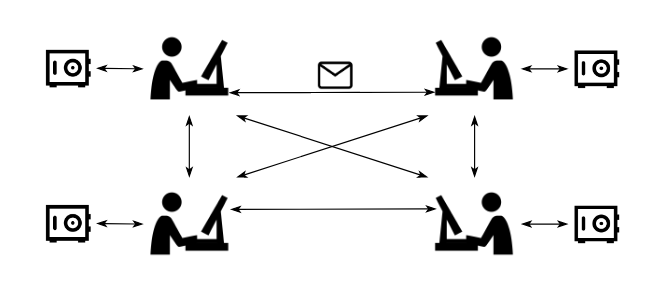
\includegraphics[width=0.7\textwidth]{./Images/main-figure.png}
    \caption{System illustration.}
    \label{fig:main-system}
\end{figure}

This section will define and detail the use cases the solution must satisfy and provide to the user. The combination of the use cases satisfy the client requirements in section \ref{chap:problem:requirements}.
Figure \ref{fig:main-system} will be used as an example and illustration for the different scenarios.

% -----------------------------------------------------
\subsection{Initial State}\label{chap:problem:scenarios:init}

The users will receive the device with a pair of asymmetric keys, a private and public, generated inside the device from fabric.
Each device will have the user's public keys, whom he wishes to communicate.
The user can request whose public keys he wants, before the device is initialized in fabric.
This allows the users to share symmetric keys between them, which they can user to begin trading data securely.
The device can also come with the symmetric keys already shared and stored in each user device.

% -----------------------------------------------------
\subsection{Authentication}\label{chap:problem:scenarios:auth}

Every user must authenticate himself, before using the device. This can be done by providing a \ac{PIN}, which the device will verify before unlocking the session for the user.
The device will come from fabric with a default authentication \ac{PIN}. The users should be allowed to change this number.

For \textbf{personal} devices, there is only one user, the owner, as illustrated by Alice and Bob in figure \ref{fig:main-system}. There is only the single authentication \ac{PIN}, which when sent to the device, unlocks the session, and the user can access its services.
For \textbf{groups} and entities, there can be multiple users, illustrated by Charlie. In this case, there are different scenarios for authentication.
The simplest is when it is not needed to authenticate the individual user, only the entity. There is only a single authentication \ac{PIN} for the entity. All the user's with permission to communicate in behalf of the entity, must know the \ac{PIN}. They only need to send the number to the device to be allowed access to its operations.

The second scenario, is when an entity wishes to authenticate each individual user with access to the device. 
This would entail a more complex process. A user will be assigned the role of administrator. For example, in the military, this could be assigned to the top ranking general. The administrator, using the \ac{PIN} from fabric, is able to register new users with their own private \ac{PIN}, access the logs of which user logged in and when, as well as, which messages they sent and received.
The registration of a new user must be done physically with both administrator and user. The administrator authenticates himself to the device, begins the registration process and allows the user to insert their name and \ac{PIN}.
It is important to note that in all scenarios, only the users or the entity is authenticated, the device does not authenticate itself to the user.

% -----------------------------------------------------
\subsection{Communications}\label{chap:problem:scenarios:comms}

For each channel of communication between individual users, groups or entities, the same symmetric key is saved in secure storage on both devices. For one channel, one key is used.
These device has a limited amount of secure storage, so only a certain amount of symmetric keys can be stored there.
When a user wants to send a secure message, the plaintext data is first sent to the device. Inside, it will secure the data using the correct symmetric key, and return it to the user. The user can then send the secured through a convenient service such as email. Only the recipient with a similar device with the same key can read the contents.

In the simplest scenario, the system allows secure communications between a limited amount of entities. Each entity, upon ordering the device, specifies which entities it wants to communicate with. For example, Alice can request a device which enables two separate channels with Bob and Charlie. Alice can also request a single channel with all three entities, in this case, only one key is required for all.
In fabric, the required keys will be generated and stored in every necessary device. When all involved entities receive their device, they can begin communications immediately.
This approach is easier to develop and implement, but is not very flexible. It has a limit on the number of communications, does not allow for the users to establish new channels of communication without return the device to manufacturing, and does not support digital signatures due to lack of asymmetric keys.

There is an approach with improved features, by including asymmetric keys in the process.
Each device has one pair of asymmetric keys stored in secure storage. This pair identifies the entity, only it possesses the private key. Symmetric keys used for communication are encrypted with the public key and be stored in plain memory. Only the private key inside the device in secure storage can decrypt these keys. This permits the storage of a practically unlimited number of symmetric keys, since the secure storage size constraints are not a factor.
With the addition of these type of keys, digital signatures are available and users can communicate with new entities. This also opens the possibility for the symmetric keys to have an expiration date, to avoid overuse, and reduce the possibility of being compromised. When they expire, new ones can be exchanged.

% -----------------------------------------------------
\subsection{New Channels of Communication}\label{chap:problem:scenarios:keys}

The users can establish new channels of communication with new users, or in some cases, users with already existing channels. This assumes the devices securely store a private and public key.
When a new user wants to establish secure communications with a new user or a group, in possession of an identical device, he must share his public key with the user, ideally physically to ensure no one is impersonated. After this, they can securely share symmetric keys. This is achieved by just sending a message to the device, indicating you want to generate a new symmetric key, to communicate with a specific user. The device saves the new key inside the device, and secures it with its private key and the other user's public key. The key can then be sent just like any other message. When the key is stored in both devices, secure communication is achieved.

There are cases where existing keys might need to be revoked due to suspicion of being compromised, or simply because their validity has expired, and new keys need to be exchanged. In this case, with the device already in possession of the other user's public key, and similarly to the previous scenario, a new symmetric key is generated and stored with public-key cryptography in the device. The old key is erased from memory, and the new one is returned to the user, along with a message for the other entity to delete the old key. After the individual shares the key and message with the other entity, the key is likewise stored in their device, and the old one deleted.

% If Printing on DOUBLE SIDED pages, the second page should be white.
% Otherwise, comment the following command:
% \cleardoublepage
%
%Chapter 3
% #############################################################################
% This is Chapter 3
% !TEX root = ../main.tex
% #############################################################################
% Change the Name of the Chapter i the following line
\fancychapter{Problem Definition}
\cleardoublepage
\label{chap:problem}

This chapter defines the problem, the client requirements and lists the necessary services of a potential solution, which successfully addresses the problem.
First, some context surrounding the problem is given. Next, the profile of the target users is described. The following section lists the client requirements the solution must provide.
Then, it will shed the light on some essential concepts, to understand the services that need to be implemented. Lastly, it details some possible use case scenarios.

% -----------------------------------------------------
\section{Context}\label{chap:problem:context}

As discussed before, the same computers commonly used for communications and information storage are exploitable by attackers, and can cause minor inconveniences, to severe repercussions, such as, losing your confidential data to malicious parties.
This work focuses on an interesting approach to improve security, by adding another layer of security to communications, through the addition of a device, independent of the user's computer. The device is responsible for the security of sensitive data and communications.

% -----------------------------------------------------
\subsection{Entities}\label{chap:problem:entities}

These type of devices are especially relevant to people with high responsibility jobs, that handle very sensitive information, which have dire consequences if they are lost, corrupted or leaked.
Some examples are government officials who handle confidential information pertaining a country, company executives, such as the CEO with access to company secrets, diplomats who manage confidential treaties, and military officers who have access to information critical to national security.
Not just individuals could have an interest in these systems. A device can be assigned to a group of people representing an entity. For example, in the military, a device can be assigned to the navy, one to the infantry and so on. Any ranked officer, or person with a certain level of authority, could use the navy's device, to communicate with other entities, in behalf of the navy.

\subsection{Devices}\label{chap:problem:devices}

There are dedicated devices currently on the market, designed to secure communications and store private data.
These type of devices have physical tamper-resistant measures against attackers, who wish to read the device's information. They also provide fail-safe mechanisms in case of an attack.
\ac{HSM} is a high grade device, with more computational power and larger storage capacity for secrets.
Smart Cards, provide secure and portable tamper-resistant storage. They have lower processing power, and a smaller memory. They have a lower cost, so can be produced in bulk and easily replaced.
Because of these features, they are widely used in the retail, healthcare, communication and government industries.

% -----------------------------------------------------
% -----------------------------------------------------
\section{Requirements}\label{chap:problem:requirements}

To effectively address the problem, there are several high-level requirements the solution must adhere to:
\begin{itemize}
	\item Devices should be distributable to individuals or entities, with more than one person;
	\item The system must allow communications between individuals, representing themselves or an entity;
	\item The system must be responsible for securing all communications against any attacks;
	\item The device should be independent from the user's personal computer;
	\item Users should be able to establish secure communications with new and existing entities;
	% \item New secure connections should be created, if existing communications are suspected to be compromised;
	\item It should provide an easy-to-use interface for non-technical people;
	\item It should have a relatively low cost, to allow distribution of several devices among multiple people;
	\item Only authorized individuals should be able to use the device.
\end{itemize}

These client requirements need to be translated into slightly more technical and tangible requirements. In order to secure communications, the solution should guarantee confidentiality, integrity and authentication.
Additionally with asymmetric keys, the system can provide non-repudiation to documents or files, by means of qualified digital signatures.
The device must securely store all keys, and perform all cryptographic operations pertaining the security of communications. Keys must never be exposed unencrypted to the outside.
Additionally, the device should have physical tamper-resistant measures and mechanisms in place, in case of an intrusion, such as, permanent erasure of all sensitive data. 
This means that even if an attacker is in possession of the physical device, it should be extremely difficult to extract any information from it.
The solution should work with a plethora of devices, in order to increase the adoptability of the solution among clients, or to be easily adapted in other projects.
The system should provide an application on the user's computer, which communicates with the physical device, and offers a simple interface to the its services, for the average non-technical user.
The system should use a common connection solution, e.g. \ac{USB} cable, between the computer and device, to further increase adoptability.
In addition, the system should perform the services in a reasonable time, to minimize the wait, and improve the user experience.

% -----------------------------------------------------
% The solution should follow the \ac{PKCS} \#11 standards, to strengthen its security requirements.
% This is where the widely established standard \ac{PKCS} \#11 is again relevant. It allows operations to be standardized across different devices, increasing the range of supported devices.
% By implementing the system in accordance with these guidelines, it will have a higher device interoperability.

% -----------------------------------------------------
% -----------------------------------------------------
\section{Use Case Scenarios}\label{chap:problem:scenarios}

This section details use case examples the solution must cater to. Figure~\ref{fig:user:data-service} will be used as an example and illustration for the scenarios.

% -----------------------------------------------------
\subsection{Authenticating the User}\label{chap:problem:scenarios:auth}

Every user must authenticate himself before using the device. This can be done by providing a \ac{PIN}, which the device will verify, before unlocking the user's session.
The device will come from fabric with a default authentication \ac{PIN}. The users should be allowed to change this number.
For personal devices there is only one user, the owner, as illustrated by Bob in figure~\ref{fig:user:data-service}. There is only a single authentication \ac{PIN}, which when sent to the device, unlocks the session, and the user can access its services.
For groups and entities there can be multiple users, illustrated by Alice. In this case, there are different scenarios for authentication.
The simplest is when the individual user does not need to authenticate himself, only the entity. There is only a single authentication \ac{PIN} for the entity. All the user's with permission to communicate in behalf of the entity, must know the \ac{PIN}.
The second scenario, is when an entity wishes to authenticate each individual user, with access to the device. 
This entails a more complex process. A specific user is assigned the role of administrator. For example in the military, this could be assigned to the top ranking general. The administrator, using the administrator \ac{PIN}, is able to register new users with their own private \ac{PIN}, access the logs of which user logged in and when, as well as, which messages they sent and received.
The registration of a new user can be done physically with both administrator and user present. Afterwards, the registered user can use their credentials to authenticate himself, and use the device to communicate, in behalf of the entity.
It is important to note that in all scenarios, only the users or the entity is authenticated, the device does not authenticate itself to the user.
% The administrator authenticates himself to the device, begins the registration process and allows the user to insert their name and \ac{PIN}.

% -----------------------------------------------------
\subsection{Secure Communications}\label{chap:problem:scenarios:comms}

%% SECURE COMMUNICATIONS %%
The main goal of the system is to enable secure communications. Communications can be setup between two or more entities. For each configured communication, the same symmetric key is securely stored in each device. One key per communication.
For a user to send secure data, first he authenticates himself to the device, then sends the data to it. The device will return it secured. The user can then send it through a convenient offline service such as email, or an online chat service. Only a recipient with a similar device and the same key can read the original contents.

\begin{figure}[h!]
    \centering
    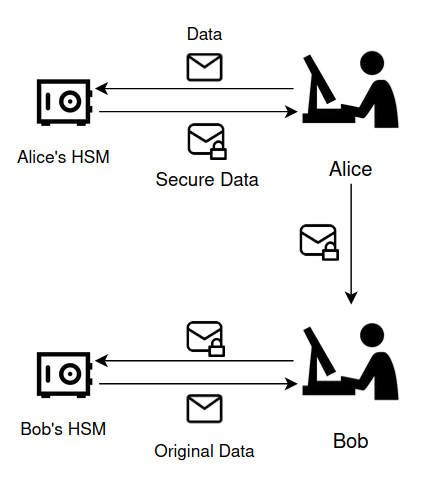
\includegraphics[width=0.7\textwidth]{./Images/user-data-service.png}
    \caption{Secure data exchange service example using internal keys}
    \label{fig:user:data-service}
\end{figure}

%% USAGE EXAMPLE %%
A possible usage example of secure data exchange between two users, Alice and Bob, is depicted in figure \ref{fig:user:data-service}. Firstly, Alice forwards the data, to be sent securely to Bob, to the device and the device returns the data secured with an internal key. Then, Alice can forward the result to any entity with the same internal key in their device, through a chat application, e-mail or other convenient service.
Upon receiving the secure message from Alice, Bob sends it to the device, and receives the original message back.
This service must prevent any third party from gaining access to the data, or altering the message. The receiver can be confident of the data's origin. It could not have been sent by any malicious entity.

%% INITIAL STATE, FABRIC CONFIGURATION %%
%% COMMUNICATION CHANNELS LIMIT %%
Each entity, upon ordering the device, should be able to specify which entities it wants to communicate with.
For example, Alice can request a device which enables two separate communication channels with Bob and Charlie, separately. Alice can also request a single channel with all three entities. In this case, only one shared key is required for all.
Before devices are delivered, the keys will be generated and stored in the necessary device. When all involved entities receive their device, they can begin secure communications immediately.
The device should not have a practical limit on the amount communication channels it can establish. This means it should have a reasonable amount of key storage space, for communications with enough different entities.
If the device's secure storage is limited, then a solution using symmetric or asymmetric keys to secure all other keys on a higher capacity non-volatile memory.
This gives entities the flexibility needed to communicate with the number of entities they choose.

%% QUALIFIED DIGITAL SIGNATURES %%
Another possible use case scenario is the inclusion of a pair of asymmetric keys, generated inside each device, and never exposed to the outside. This allows the generation of qualified \textbf{digital signatures}, which can legally represent the entity.
Then, when a user wishes to generate a signature for a piece of data, he must send the data to the device, which computes and returns the qualified signature.
% Each device has a pair of asymmetric keys stored in secure storage, generated inside the device from fabric. These keys allow the storage of a practically unlimited number of symmetric keys in non-volatile memory.
% This feature is useful in other situations. There are cases where existing symmetric keys might need to be revoked, due to suspicion of being compromised, with new ones generated and shared.
% Another case is if the symmetric key has an expiration date, when it expires, new keys need to be exchanged.

% Finally, when using asymmetric keys, beyond providing authentication to the communications, the data sender can be authenticated to the receiver, using the entities private key stored in the device.

% -----------------------------------------------------
\subsection{New Communications}\label{chap:problem:scenarios:keys}

%% REASONING FOR SERVICE %%
%% SERVICE PRESENTATION %%
The operations described so far provide a usable and functional system to organizations and users, but it is not very flexible. It does not allow users to communicate with new entities, without returning the device to manufacturing, to be equipped with the necessary information.
To avoid this, a service should be available to users with production devices in their possession, to securely trade data with another entity with an identical device, which the device previously could not. It should be easy to provide the functionality without burdening the user with additional responsibility.
A possible solution is the inclusion of a control station, where entities originally collect their devices. Each device is delivered with its own communication channel with the control station. This station is effectively treated as a special entity.
Whenever users wish to communicate with another user, they can send a list of entities they intend to communicate with to the station, secured with the data exchange service. The control station subsequently supplies the user with the necessary information, to be imported in their device.

\begin{figure}[h]
    \centering
    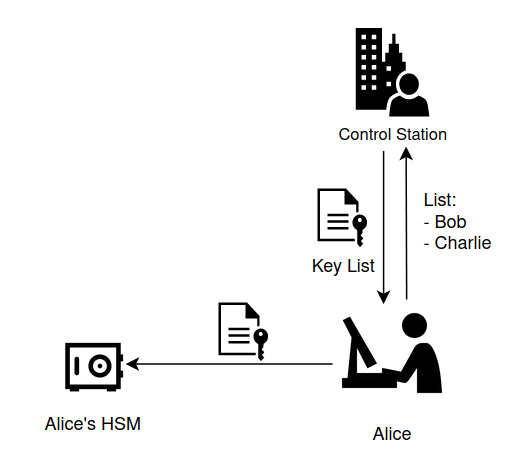
\includegraphics[width=0.65\textwidth]{./Images/user-import-service.png}
    \caption{Import key list to device usage example}
    \label{fig:user:import-service}
\end{figure}

%% USAGE EXAMPLE %%
%% ADVANTAGES / POSSIBILITIES %%
A use case scenario of this service is depicted in figure \ref{fig:user:import-service}.
Alice forwards the list with the names of entities to the control station, which returns the key list to Alice. The list can be forwarded to the device, where the new keys are stored.
Alice can then start communications with Bob and Charlie, using the secure data exchange service, as soon as everyone imports the list into their respective devices.
The service offers the possibility of setting up a regular communication update schedule. It grants the flexibility of key revocation when needed, data exchange with new entities, as well as updating communication keys, which have reached their expiration date, with no additional complexity to the user.
A regular update schedule, adds longevity to the system. It avoids overuse, and reduces the possibility of compromised connections. When keys reach the expiration date, new ones can be distributed.
A less cumbersome possibility for the user, is whenever an entity is added to system and receives their device, the station delivers a message to each entity, with the updated key list. The list can be imported by each user if needed.

% The list can be sent using an offline service such as email. Every time a new entity is added to the list, the station sends a new email with the updated list. Each entity can get access these updates when they need it.

% Each month an entity can hand over a list of the entities it wishes to communicate with to the control station, which will accordingly yield the corresponding key set, as pictured in figure \ref{fig:user:import-service}.
% Each entity only needs to forwards the list to the device, and the new keys are immediately stored and ready to be used.


% The list can be provided at the manufacturing control station, when the device is delivered.
% Afterwards, there are two options to distribute the list. When the list is updated with new entities, a member of the entity will physically go to the station, to retrieve it.
% Alternatively, the entity will receive the device with the necessary keys to securely communicate with the control station. When an entity needs the list, it will be supplied for them by the control station. In this scenario, the control station can be thought of as a special entity.

% Adding to the previous scenario with asymmetric keys, users will be able to establish secure communications with new entities. This is achieved by distributing a list of available entities to communicate with.
% When and individual, e.g. Alice, wants to establish communications with a new entity, such as Bob, she needs to get Bob's key from the received list. Then they can securely trade a new key, and begin communications.

% -----------------------------------------------------
% -----------------------------------------------------
\section*{Summary}\label{chap:problem:summary}

This chapter defines the context for the addition of a device, independent of a personal computer, which secures communications between entities, such as the military or government.
The fundamental and non-technical requirements for an adequate solution were defined, such as, its characteristics, capabilities and usability. In short, the system should be composed of a user-friendly and low cost device, easily distributed among individuals or groups, and provide secure communications between them.
Several possible use case scenarios for the system were identified.
The system could be used to authenticate a user to the device, to allow access to its secure communication capabilities. The system must allow communications between entities with identical devices, by the means of a personal computer connected to the device, which secures the messages before transmission.
The system could also allow the establishment of communications with new entities, by employing a control station which, when necessary, distributes the essential information among all entities, to allow new secure communication channels.

% If Printing on DOUBLE SIDED pages, the second page should be white.
% Otherwise, comment the following command:
% \cleardoublepage
%
%Chapter 4
% #############################################################################
% This is Chapter 4
% !TEX root = ../main.tex
% #############################################################################
% Change the Name of the Chapter i the following line
\fancychapter{Architecture}
\cleardoublepage
% The following line allows to ref this chapter
\label{chap:arch}

The objective of the system was to develop a device in a box format to enable users to establish safe channels of communication. This is achieved with a safe and secure device which is personal to each individual. In order to secure the communications between users, the device saves the user's sensitive data, such as keys, and performs all security critical operations.
The system is designed so that each user has it's own physical box.

% -----------------------------------------------------
% -----------------------------------------------------
\section{Components}\label{chap:arch:components}

The system architecture, depicted in figure~\ref{fig:components}, is composed of two main components: the physical box which responsible for securing the data, and the client software on the user's computer, which communicates with the box.

\begin{figure}[h]
    \centering
    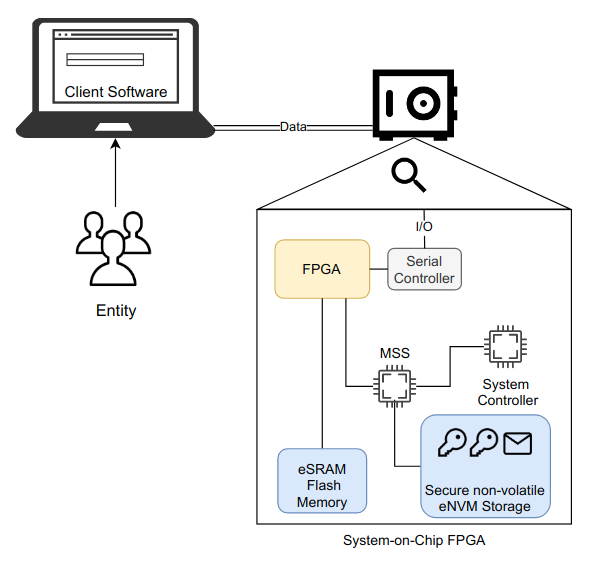
\includegraphics[width=0.7\textwidth]{./Images/main-components.png}
    \caption{System Components}
    \label{fig:components}
\end{figure}

The client software sends and receives data through the device's serial I/O port, which exposes an \ac{API} to access its operations.
With this connection the entity can signal the device to perform the desired operations, through the client software.
The device integrates a \ac{FPGA}, \ac{MSS}, secure eNVM storage and flash memory for configuration. The \ac{MSS} has an embedded ARM processor, connected to the system controller which provides several cryptographic services. The secure eNVM allows storage of keys, data and secure boot code.
The \ac{MSS} uses the keys stored in the eNVM, with the cryptographic algorithms in the system controller.

% -----------------------------------------------------
% -----------------------------------------------------
\section{Operations}\label{chap:arch:ops}

This section will define and describe the system architecture. It is structured starting with the authentication and then the system operations, divided by types.
The architecture will be explained, using the scenarios in section \ref{chap:problem:scenarios}.

For the user to be able to perform operations, he first must authenticate himself to the device. The device will come from fabric with a default authentication \ac{PIN}. To authenticate himself to the device, the user sends a \ac{PIN} through the software, the device then compares it to the authentication number stored inside. To protect the number it can be either stored in the secure eNVM if there is enough space, or in other non-volatile memory, signed with the device's public key. Once authenticated, the session will be unlocked, and the user will be able to perform operations.
If only the entity is authenticated, not the individual, a single \ac{PIN} is used for all authentications.
If instead the individual is authenticated, the user will send the registered name and the number, and the device will use the name to identify the correct number.

After authentication, the operations that can be performed, are split in three types:
\begin{itemize}
    \item Administration operations configure authentication and communication parameters;
    \item The secure communication operations provide the cryptographic services to secure communications;
    \item Communication management operations manage the keys used to secure connections.
\end{itemize}

% -----------------------------------------------------
\subsection{Administration}\label{chap:arch:ops:admin}

The administration operations will allow the user to manage the authentication related parameters.
For the first scenario, the only operations of this type is to change the authentication \ac{PIN}. The user sends the number to the device, and it will be securely saved inside it. The device will be initialized from fabric with a default \ac{PIN} which must be supplied to the user. Before performing any operation the user should change his PIN to begin secure communications.

The second scenario has an administrator role and a user role. Each user has its own \ac{PIN}. The administrator, beyond changing the authentication number, can register new users. To register a new user, both administrator and new user need to be physically together with the device. The administrator authenticates himself to the device, begins the registration process and allows the user to insert their name and \ac{PIN}. After this the user can login with name and number, and access all secure communication operations, as well as changing their own \ac{PIN}.

% -----------------------------------------------------
\subsection{Secure Communication}\label{chap:arch:ops:comms}

The main operations will be responsible to secure the communications between users. These operations will grant the confidentiality, integrity, authentication and non-repudiation services to communications.

Th objective of communications with \textbf{confidentiality} and \textbf{authentication} is to send and receive data securely, to and from the device. The user sends plaintext data, and the device returns it encrypted and authenticated with the symmetric key stored inside the device, of the corresponding connection. In the equivalent operation reversed, the ciphertext is sent to the device, and the plaintext is returned.
Both operations are pictured in figures~\ref{fig:arch-encrypt} and~\ref{fig:arch-decrypt}.

\begin{figure}[h]
	\centering     %%% not \center
	\subfigure[Encrypt and authenticate data with K1 key]{\label{fig:arch-encrypt}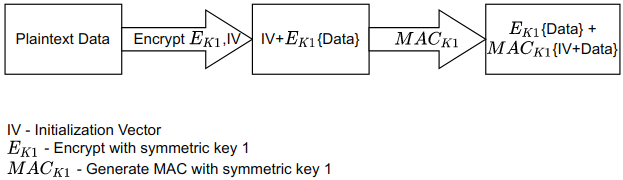
\includegraphics[width=1\textwidth]{./Images/arch-encrypt.png}}
	\subfigure[Decrypt data and verify authentication with K1 key]{\label{fig:arch-decrypt}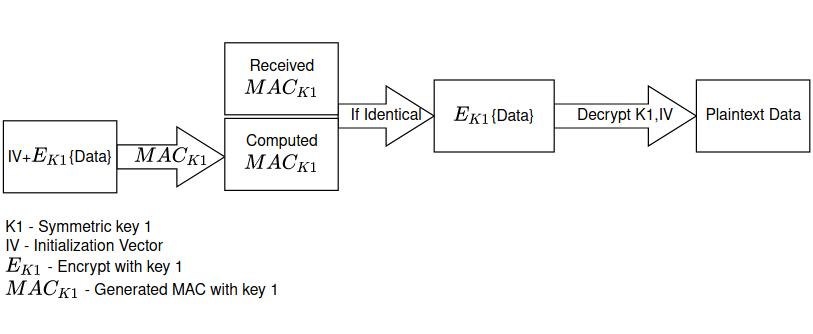
\includegraphics[width=1\textwidth]{./Images/arch-decrypt.png}}
	\caption{Procedure to secure data with authentication and confidentiality}
\end{figure}

Beginning with figure~\ref{fig:arch-encrypt}. The plaintext data sent to the device is first encrypted with the symmetric key \textit{K1}, using a randomly generated \ac{IV}. Then a \ac{MAC} is generated from the encrypted data and \ac{IV}, using the symmetric key. All fragments of information (IV, ciphertext, MAC) are returned to the user, and the user can then send it to other entities in possession of the used \textit{K1} key.
Following with figure~\ref{fig:arch-decrypt}, when a device receives the ciphertext, it decrypts the data using the same \textit{K1} key and received \ac{IV}. Then it computes the MAC of the received \ac{IV} appended with the decrypted data. If the computed and received \ac{MAC} are identical, the data is authenticated.

Qualified digital signatures provide \textbf{non-repudiation} to a piece of data, using the private key generated inside the box. The user sends the data to the box, and the subsequent signature will be returned as pictured in figures~\ref{fig:arch-ds} and~\ref{fig:arch-ds-verify}.

\begin{figure}[h]
	\centering     %%% not \center
	\subfigure[Alice generates signature of a document]{\label{fig:arch-ds}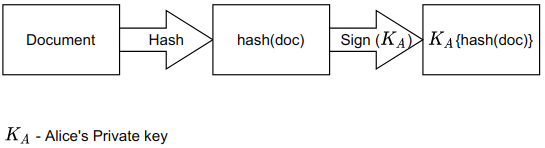
\includegraphics[width=0.7\textwidth]{./Images/arch-ds.png}}
	\subfigure[Bob verifies the signature of the document]{\label{fig:arch-ds-verify}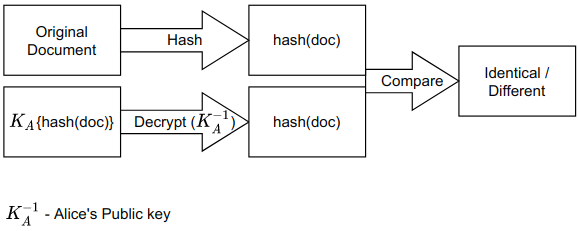
\includegraphics[width=0.7\textwidth]{./Images/arch-ds-verify.png}}
	\caption{Procedure to generate and verify a qualified digital signature}
\end{figure}

The signature is generated by calculating the hash of the data, and signing the digest with the device's private key. To verify a signature (figure~\ref{fig:arch-ds-verify}), the device decrypts the hash with the signer's public key. Next, it computes the hash of the original document, and compares both hashes. If they are identical, the qualified signature is valid.

% -----------------------------------------------------
\subsection{Communication Management}\label{chap:arch:ops:key}

These operations will manage the needed keys to support secure communications, digital signatures and create new secure connections.
Supported key management operations are: symmetric key generation, symmetric key revocation, if communications are suspected to be compromised, and importation of other entities' keys.
These operations are only available in the scenario where each device has a pair of asymmetric keys.

An entity receives their device, prepared to communicate with other entities, and a list of information of other entities, available to create communications. This information, namely the entities public key, needs to be imported into the device's non-volatile memory. It does not need to be secure storage.
After the key is imported, a secure connection with a new entity can be established, by sharing symmetric keys.
For an entity to communicate with a new entity, their device will generate a new symmetric key and store it either in secure storage, or in non-volatile memory, encrypted with the device's public key. Figure~\ref{fig:arch-new-key} illustrates the procedure Alice's device goes through to share a new key with Bob.

\begin{figure}[h]
	\centering     %%% not \center
	\subfigure[Alice generates key]{\label{fig:arch-new-key}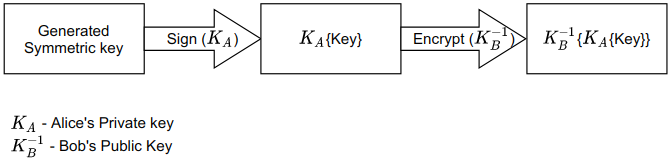
\includegraphics[width=0.8\textwidth]{./Images/arch-new-key.png}}
	\subfigure[Bob saves key]{\label{fig:arch-save-key}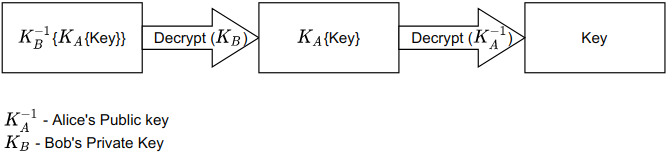
\includegraphics[width=0.8\textwidth]{./Images/arch-save-key.png}}
	\caption{Alice generates a new key to share with Bob}
\end{figure}

The key is first signed with the sender's private key, which is stored in the device's secure storage, and then ciphered with the receiver's public key, which was imported before. Portrayed in figure~\ref{fig:arch-save-key}, Bob's device decrypts the message using its private key, and decrypts it again with Alice's public key. Finally the key is securely stored in the device, and both entities can subsequently establish secure communications.

When a symmetric key is revocated, due to reaching its expiration date, or from being compromised, entities can generate a new one, using the aforementioned procedure.

% If Printing on DOUBLE SIDED pages, the second page should be white.
% Otherwise, comment the following command:
% \cleardoublepage
%
%Chapter 5
% #############################################################################
% This is Chapter 5
% !TEX root = ../main.tex
% #############################################################################
% Change the Name of the Chapter i the following line
\fancychapter{Implementation}
\cleardoublepage
% The following line allows to ref this chapter
\label{chap:implementation}

This section will build on the system architecture. It describes the communication protocols, standard and libraries chosen to implement the operations. It will start by clarifying important assumptions. Then it will start with the initial state specifications, and finish by defining the protocol for each operation, introduced in chapter \ref{chap:arch}.

% -----------------------------------------------------
% -----------------------------------------------------
\section{Libraries and Tools}\label{chap:implementation:tools}

The cryptographic software is running on the \ac{SoC} of a SmartFusion2 board from Microsemi, discussed in section~\ref{chap:background:computing:smartfusion}. It is an adequate device due to several components such as the required cryptographic functions in its system controller, a \ac{TRNG} essential for cryptography, secure storage for keys and anti-tampering protections.
The application was implemented using the C programming language, with the SoftConsole \ac{IDE} and libraries of the board functionalities, provided by Microsemi. The device functions as a \ac{HSM}, connected through a \ac{USB} connection to a computer.
The client software was also implemented in C, and is composed of a simple interface which allows communication through the cable, to the device.

% -----------------------------------------------------
\subsection{Cryptographic Algorithms}\label{chap:implementation:tools:algorithms}

As previously mentioned, \ac{AES} is a popular symmetric-key standard. The security of \ac{AES}-\ac{GCM} in hardware is considered to be unsurpassed by any authenticated-encryption scheme~\cite{aesmodes}.
Unfortunately, the SmartFusion2 board, does not support this encryption algorithm. Therefore the solution is a combination of an encryption algorithm with an authentication scheme. The board supports the \ac{AES} encryption modes for confidentiality, either 128 or 256 bits: \ac{ECB}, \ac{CBC}, \ac{OFB} and \ac{CTR}. CTR mode is the most favourable option because of its efficiency and security, assuming the IV is unique for each message.
For authentication, the board supports \ac{HMAC} with the \ac{SHA}-256 hash function, which uses a 256 bit symmetric key and generates a 256 bit code. For combining the CTR and HMAC algorithms, studies have shown that a combination of secure encryption and secure MAC must use the encrypt-then-MAC method~\cite{encryptmacorder}.
When choosing key sizes, taking into account the limited storage capacity of the board, a smaller key size, but still secure is preferred. \ac{AES} guarantee both 128 and 256 bit security, with 128 and 256 bit keys. According to the \ac{NIST} recommendations~\cite{nistRecommendations}, both 128 and 256 bit security, are expected to be secure from 2031 and beyond. Since \ac{AES}-128 guarantees adequate security for the foreseeable future, and is smaller, it is the chosen option.
The \ac{HMAC}-\ac{SHA}-256 algorithm needs a 256 bit key, different from the one used with encryption, to ensure the best security practices. Thus, for every communication, a 128 bit key for encryption and a 256 bit key for authentication is used. In total, a 384 bit symmetric key.
The used algorithm for public-key cryptography is \ac{ECC} with 384 bit private and public keys, the only one supported by the board, which guarantees 128 bit security, same as \ac{AES}-128.

% -----------------------------------------------------
\subsection{Device Standardization}\label{chap:implementation:tools:standardization}

The solution should support a plethora of devices, as it will increase the adoptability of the solution among clients. This entails the use of a widely established protocol, which clearly defines a set of functions and standards the system should follow.
The \ac{PKCS} \#11 standard will be utilized to fulfill this requirements. It allows operations to be standardized across different devices, increasing the range of supported devices. By implementing the system in accordance with these guidelines, it will have a higher device interoperability. Additionally, it allows the application to use, create and modify objects, without exposing them to its memory.

% -----------------------------------------------------
% -----------------------------------------------------
\section{Protocol}\label{chap:implementation:protocol}

All data and operations will flow through a serial connection between the client software in the individual's computer and the physical box. A communications protocol needs to defined, in other for this communication to occur.
This section will explain and define the communication protocols between both the client application and the hardware device in detail. For each operation, it will describe its goal, the different phases, what data is traded in each phase and why.

% -----------------------------------------------------
\subsection{Initial State}\label{chap:implementation:protocol:initial-state}

The device will come from fabric configured and prepared with the necessary keys depending on two scenarios. In the simpler scenario, the device comes with the symmetric keys already shared and stored in each entities' device. They can begin to communicate immediately, with no setup necessary.
In the other scenario, the entities will receive the device with a pair of asymmetric keys, a private and public, generated inside the device from fabric. Each device will have the user's public keys, whom he wishes to communicate. The entity can request whose public keys he wants, before the device is initialized in fabric. This allows the users to share symmetric keys between them, which they can user to begin trading data securely.

% -----------------------------------------------------
\subsection{Authentication Protocol}\label{chap:implementation:protocol:auth}

Before executing any operation the user must authenticate himself to the device.
Figure~\ref{fig:protocol:authentication} depicts the authentication protocol.

\begin{figure}[h!]
	\centering
	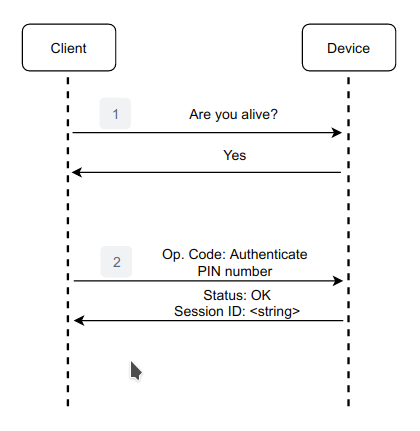
\includegraphics[width=0.45\textwidth]{./Images/authentication.png}
	\caption{Authentication Protocol}
	\label{fig:protocol:authentication}
\end{figure}

The user initiates by sending a message to check if the device is alive and connected to the computer. After the device responds with an acknowledge, the user software sends the authentication \ac{PIN}. The device will respond with a status parameter indicating failure or success. When it is successful, the session will be unlocked, allowing the user access to the main operations.

% -----------------------------------------------------
\subsection{Administration Protocol}\label{chap:implementation:protocol:admin}

There is only one administration operation, changing the authentication \ac{PIN}, pictured in figure~\ref{fig:protocol:change-PIN}.
The user initiates by sending the change \ac{PIN} operation code, and the new \ac{PIN} number. The device responds with the return status of the operation.

\begin{figure}[h!]
	\centering
	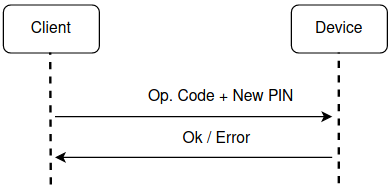
\includegraphics[width=0.4\textwidth]{./Images/change-PIN.png}
	\caption{Protocol to Change Authentication PIN}
	\label{fig:protocol:change-PIN}
\end{figure}

% -----------------------------------------------------
\subsection{Secure Communications Protocol}\label{chap:implementation:protocol:comms}

The protocol for operations which secure communications will be defined here. It covers the encryption and authentication operation, which enables secure communications and non-repudiation through qualified digital signatures.
The protocol to encrypt and authenticate data illustrated in figure~\ref{fig:protocol:data-exchange} consists of four phases.

\begin{figure}[h!]
	\centering
	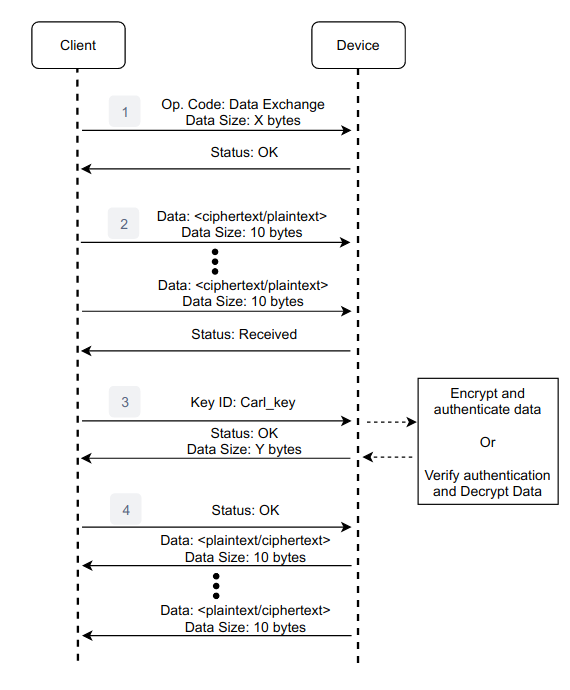
\includegraphics[width=0.6\textwidth]{./Images/data-exchange.png}
	\caption{Encryption+Authentication Protocol}
	\label{fig:protocol:data-exchange}
\end{figure}

It starts with the user sending the operation code and the data size. The box will respond with an OK message signaling the client application can begin to transmit the data. A maximum of X bytes per message can be transmitted. Each message contains a part of the data and the size of the data in that packet. When the transmission ends, the device confirms its reception.
In the third phase, the client software sends the ID of the symmetric key used to encrypt and authenticate communications with. The box will execute the cryptographic operations and return a status message and the encrypted data size.
When the client acknowledges its reception, the encrypted data with the \ac{MAC} and \ac{IV} parameters appended, will be sent back, one message at a time.

The protocol to decrypt and verify data authentication is very similar to the previous one, and is also pictured in figure~\ref{fig:protocol:data-exchange}. The differences are in phase three, after the ciphertext and symmetric key ID are transmitted, the device will decrypt and authenticate the data. It returns the operation status and the decrypted plaintext size if it was successful. It ends by transmitting the plaintext in the fourth phase to the client software.

\hfill
\hfill

The next protocols are relating to the generation and verification of digital signatures.
The designed protocol for generation is represented in figure~\ref{fig:protocol:signature-generate}.
%% ------------
\begin{figure}[h!]
	\centering     %%% not \center
	\subfigure[Generation Protocol]{\label{fig:protocol:signature-generate}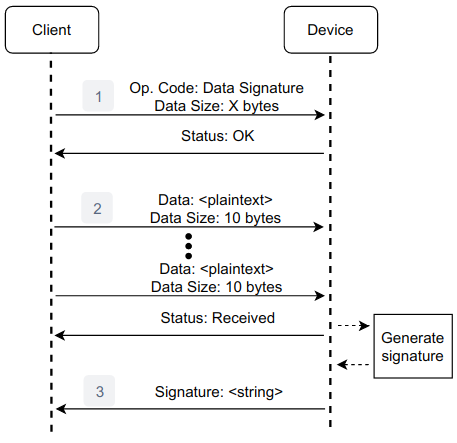
\includegraphics[width=79mm]{Images/signature-generate.png}}
	\subfigure[Verification Protocol]{\label{fig:protocol:signature-verify}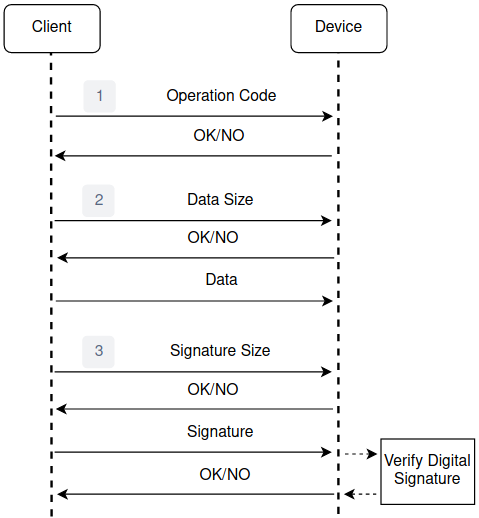
\includegraphics[width=79mm]{Images/signature-verify.png}}
	\caption{Digital Signature Generation Protocols}
\end{figure}

The user initiates by sending the operation code and the plaintext data size.
When the box responds with an OK message, the user transmits the data to be signed, one message at a time.
In possession of the data, the device will generate the digital signature using the device's private key. When finished the signature is sent back to the user.

The protocol for verifying digital signatures is pictured in figure~\ref{fig:protocol:signature-verify}.
After the user sends the operation code, and the box responds with an OK message, the user transmits the data, used by the signer to generate the signature, one message at a time.
When done, the user also sends the signature and the name of the signer, so the device knows what public key to use to verify the signature.
Then, the device will verify the digital signature using the signer's public key, the data and the signature. The result will be sent back to the user.

% -----------------------------------------------------
\subsection{Communication Management Protocol}\label{chap:implementation:protocol:key}

The protocols for the communication management operations are detailed next. The operations are importation of public keys from the list provided to entities, generation of new symmetric keys and storage of newly received symmetric keys.
The protocol to import public keys is pictured in figure~\ref{fig:protocol:import-pub}.

\begin{figure}[h]
	\centering
	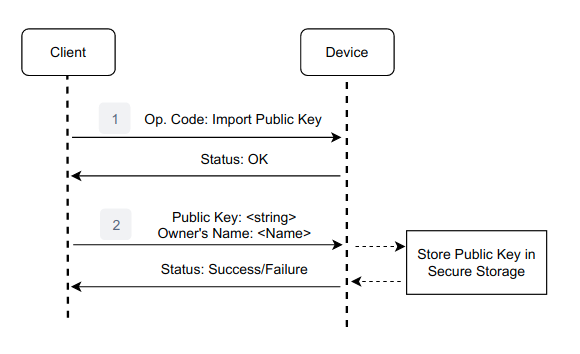
\includegraphics[width=0.5\textwidth]{./Images/import-pub-key.png}
	\caption{Import Public Key}\label{fig:protocol:import-pub}
\end{figure}

Like previous protocols, it starts with the user sending a message with the operation code, indicating he wants to import someone's public key.
After the device responds with an OK signal, the user sends the public key, and the name of the public key's owner.
The device stores the key, associated to the owner's name, and informs the client software of the operation's success or failure.

\hfill
\hfill

%% -------------------------------------
Just like digital signatures, entities can share symmetric keys between each other if they each others public keys are stored in their devices. If not, they must first import them into their respective devices.
The protocol to generate a new symmetric key, and secure it to be shared with other entities is detailed in figure~\ref{fig:protocol:new-key}.

%% --------------------------
\begin{figure}[h]
	\centering     %%% not \center
	\subfigure[Generate key]{\label{fig:protocol:new-key}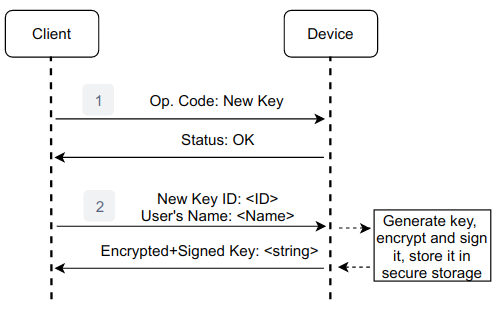
\includegraphics[width=79mm]{./Images/new-key.png}}
	\subfigure[Save key]{\label{fig:protocol:save-key}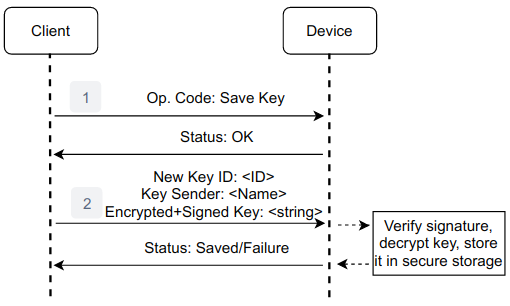
\includegraphics[width=79mm]{./Images/save-key.png}}
	\caption{Protocols for sharing keys}
\end{figure}

After both sides trade the operation code and OK status, the user sends the key ID, which will identify the symmetric key, and the name of the entity it will be shared with, so the device knows which public key to use to secure the key.
A new symmetric key will be generated and saved in the device's secure storage, with the key ID sent by the client application. The device encrypts and signs the key with public-key cryptography, and sends it back to the application, one message at a time. The user can then securely share the key with the other entity.

The protocol for the other user to save the newly received symmetric key, and store it inside their device is in figure~\ref{fig:protocol:save-key}.
After the operations code is sent and the OK signal is returned, the user sends the key ID, the name of the key sender, and the encrypted and signed key.
Then, the device verifies the signature and decrypts the key, subsequently saving it in the device's secure storage along with other symmetric keys already present.

% If Printing on DOUBLE SIDED pages, the second page should be white.
% Otherwise, comment the following command:
% \cleardoublepage
%
%Chapter 6
% #############################################################################
% This is Chapter 6
% !TEX root = ../main.tex
% #############################################################################
% Change the Name of the Chapter i the following line
\fancychapter{System Evaluation}
\cleardoublepage
% The following line allows to ref this chapter
\label{chap:evaluation}

This chapter outlines the system evaluation. It is evaluated regarding performance and fullfilled requirements from the previous report and chapter ~\ref{chap:problem}.
The performance tests discusses the objective, tests configuration, results and conclusions.
% -----------------------------------------------------
% -----------------------------------------------------
\section{Communications Performance}\label{chap:evaluation:comms}

Firstly, the performance of the communication channel was tested. Beyond testing the channel performance, it allows to test the performance of the individual services without the communication component. 
The client interface and HSM device communicate through a \ac{UART} serial port.
The performance metrics measured are the average time to transmit data and channel throughput.

% -----------------------------------------------------
\subsection{Testing configuration}\label{chap:evaluation:comms:config}

Only two program are running on the computer while performing the tests, the client program and the SoftConsole IDE needed to run the code on the smartfusion board.
The serial port UART connection is configured with 115200 bit baud rate, 8 data bits, no parity bits and one stop bit.
The elapsed time is measured through two calls to the function gettimeofday() in the C library "sys/time.h".

The test was setup on the client application. The application sends a message to the device. It is sent back by the device after reception. The two calls to the time functions are performed in the client application right before sending and after receiving the original message.

The message size was varied to study the performance and scalability of the serial port. For each message size, the test is repeated thirty times and the average time is taken from all repetitions.

% -----------------------------------------------------
\subsection{Results}\label{chap:evaluation:comms:results}

\begin{figure}[h!]
	\centering
	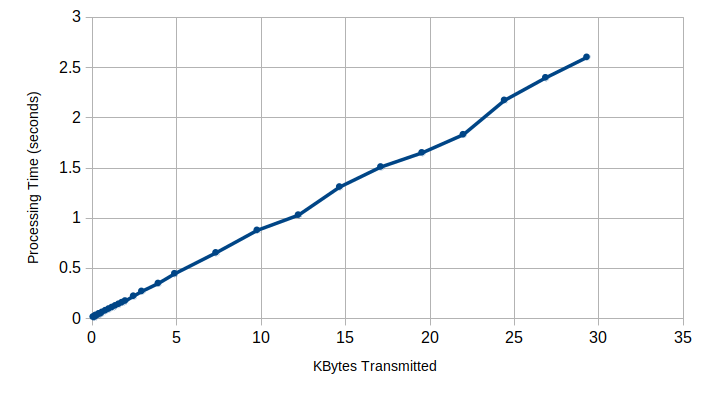
\includegraphics[width=0.85\textwidth]{./Images/comms-performance.png}
	\caption{Serial Port Communications Results}
	\label{fig:performance:comms}
\end{figure}

As seen in figure~\ref{fig:performance:comms}, the average times range from approximately 0.016 seconds with a message of 50 bytes, to 2.6 seconds with a message of 30000 bytes.
From the graph we can conclude the performance has linear scalability which is ideal for a system.
The theoretical throughput is 14400 bytes = 115200/8 bytes, calculated from the baud rate.
The experimental throughput is 3125 bytes per second with messages below 100 bytes and starts stabilizing around 12000 to 11000 bytes per second as message size increases.
From this we conclude the practical throughput is close to the theoretical, and as expected stabilizes as the message size increases, as the sample size is bigger.

% -----------------------------------------------------
% -----------------------------------------------------
\section{Services Performance}\label{chap:evaluation:services}

The objective of these tests was to measure the performance of the services implemented in the board.
The performance metric measured was the average time to finish the service, excluding the time spent on communications.

The tested services were:
\begin{itemize}
	\item Data encryption + authentication
	\item Data decryption + authentication
	\item ECDH new key generation
\end{itemize}

% -----------------------------------------------------
\subsection{Testing Configuration}\label{chap:evaluation:services:config}

The same library used to measure the time in the communication tests was used.
The time was measured at the client application before sending the message which will trigger the service at the HSM, and after it has received the result.

In order to get a real time measurement, each operation was performed 1000 times on the HSM, with the communications only done once.
From the resulting time, the predicted time spent on communications was subtracted using the data from the previous test. The result was then divided by 1000.

The data encryption and decryption operations were ran with different data sizes, in order to asses the data size impact on performance.
The ECDH key generation always uses a private and public key of the same size, so no message size variation is possible.

% -----------------------------------------------------
\subsection{Results}\label{chap:evaluation:services:results}

\begin{table}[h!]
	% \large
	\centering
	\def\arraystretch{1.5}
	\begin{tabular}{|c|c|c|c|c|} \cline{2-5}
		\multicolumn{1}{c|}{} & \multicolumn{2}{c|}{Average Time (s)}  & \multicolumn{2}{c|}{Throughput (KB/s)}\\ \hline
		\centering Data Size (bytes) & Encryption & Decryption & Encryption & Decryption \\ \hline
		79 & \textbf{0.12848} & \textbf{0.12848} & \textbf{0.6} & \textbf{0.6}	      \\ \hline
		500 & \textbf{0.12848} & \textbf{0.12849} & \textbf{3.8} & \textbf{3.8}	      \\ \hline
		1500 & \textbf{0.12853} & \textbf{0.12854} & \textbf{11.4} & \textbf{11.4}	      \\ \hline
		2000 & \textbf{0.12852} & \textbf{0.12851} & \textbf{15.2} & \textbf{15.2}            \\ \hline
	\end{tabular}
	\caption{Encryption/Decryption Performance.}
	\label{tab:data-performance}
\end{table}


The results in table~\ref{tab:data-performance} for the encryption and decryption operations are very similar due to both using the same board services, AES encryption and HMAC, but in a different order. It is also important to note AES encryption and decryption in CTR mode is essentially the same operation due the mode's characteristics.
Relating to the variation in data size, the values vary between approximately 0.1284 and 0.1825 seconds, which is a very insignificant difference. Thus we can conclude, the data size has a negligible impact on the operations performance.

\begin{table}[h!]
	\centering
	\def\arraystretch{1.5}
	\begin{tabular}{|l|l|} \cline{2-2}
	\multicolumn{1}{l|}{} & Average Time (s)  \\ \hline
		\begin{tabular}[c]{@{}l@{}}1000 reps w/o\\ enroll key\end{tabular} & \textbf{0.577155101462}     \\ \hline
			\begin{tabular}[c]{@{}l@{}}10 resp w/ \\enroll key\end{tabular}    & \textbf{1.7636150462}       \\ \hline
	\end{tabular}
	\caption{ECDH Performance.}
	\label{tab:ecdh-performance}
\end{table}


Regarding the key generation operation results in table~\ref{tab:data-performance}, two values were obtained through different methods. Due to the operation using SRAM-PUF services to enroll new keys in the eNVM memory, with limited write cycles and key slots, this operation cannot be repeated enough times to get a relevant enough sample size.
So a trade off was achieved. The operation was performed 1000 times without the key enrollment operation, meaning only the ecdh key generation algorithm and key derivation function (SHA-256).
Since the enrollment phase is presumed to be expensive, due to writing in eNVM memory, the test was also performed 10 times with key enrollment, to get an idea of its potential performance cost.

A higher time of 0.5755 without enrollment and 1.726 with, compared to the previous operations is expected due to the higher cost of operations with asymmetric keys.
However, comparing both values we can conclude saving the key in memory, has most likely the higher performance impact on the operation.

% -----------------------------------------------------
% -----------------------------------------------------
\section{Requirements}\label{chap:evaluation:requirements}

% If Printing on DOUBLE SIDED pages, the second page should be white.
% Otherwise, comment the following command:
% \cleardoublepage
%
%Chapter 6
% #############################################################################
% This is Chapter 7
% !TEX root = ../main.tex
% #############################################################################
% Change the Name of the Chapter i the following line
\fancychapter{Conclusion}
\cleardoublepage
% The following line allows to ref this chapter
\label{chap:conclusion}

This work focused on evaluating the security features of the Microsemi SmartFusion2 board, modelling its performance, and developing a proof of concept system to secure a communications channel between devices.

% -----------------------------------------------------
% -----------------------------------------------------
\section{Overview} \label{chap:conclusion:overview}

The SmartFusion2 SoC provides a varied array of security services using symmetric keys: AES with 128 and 256 bit key encryption, SHA-256, HMAC authentication with 256 bit SHA and a SHA based key derivation function. For asymmetric cryptography it offers ECDH for key generation, and additional ECC primitives, with the P-384 NIST defined curve, which can be used to implement digital signatures. Lastly, a true random number generator, a PUF based secure storage solution, tamper detection capabilities with several detection flags, and a zeroization feature with multiple recoverability options.

The prototype implemented on the device, focused on the implementation of a service which provides authentication and encryption to a TCP channel, using symmetric keys. The system is able to encrypt up to 36 KB of data using the AES and HMAC accelerators, with adequate 256 bit security. This limitation is imposed, due to the limited 80 KB of RAM.
This hurdle was overcome by implementing a continuous authenticated encryption service, using an HMAC software implementation, and taking advantage of the characteristic of the AES CBC mode.

A key generation service using asymmetric key pairs was also implemented. It generates a shared secret, using an internal private key and a public key.
The system also has a limitation in its ECC primitives. It does not provide an ECDSA implementation. In order to implement signatures, a big integer library must be included in the device. The inclusion of such a library is complex due to its tendency to be heavy in code space and the device's limited RAM memory, even when disabling error correction and detection (80 KB). 

Regarding key management, the PUF secure storage service is limited to 1000 write cycles for a predicted twenty year lifespan. To mitigate this, a key management service was developed, which stores the keys encrypted in a non volatile memory using the PUF service. This allows the update of multiple keys with only one PUF write for each update, instead of one write per key.

This work contributes with an extensive characterization of the SmartFusion2 device. It studied each security service advantage and possible trade offs. Furthermore, it models the performance of every service, providing a useful prediction of the system's behaviour. Lastly, the implemented prototype provides solid groundwork for a secure communications service, in a low cost HSM type device.

% -----------------------------------------------------
% -----------------------------------------------------
\section{Future Work} \label{chap:conclusion:future-work}

This work can be improved by implementing fully working digital signatures. To achieve this, a lightweight big integer library, with all arithmetic operations in the ECDSA algorithm is needed. It should support 48 byte integers, and have a maximum memory footprint of around 50 KB, to fit in the 80 KB of RAM with error detection and correction disabled, while keeping the secure communication and key management services enabled.
% For signature generation of unlimited data sizes, a continuous SHA implementation is necessary, since the board does not offer one.
% Future work could also test, using the secure communications service, an encrypted connection between two similar devices, running the existing prototype. The connection could be TLS encrypted, using the board to encrypt and authenticate the data, with internal symmetric keys. %This connection could be improved with a TLS implementation, using internal symmetric keys.
% Finally, the AES, SHA and HMAC cores are not side-channel protected. This includes AES, SHA-256 and HMAC. This could be improved by implementing cryptographic core's of its services using the FPGA.

% If Printing on DOUBLE SIDED pages, the second page should be white.
% Otherwise, comment the following command:
\cleardoublepage
%
% -----------------------------------------------------------------------------
% BIBLIOGRAPHY
% Add the Bibliography to the PDF table of contents (not the document table of contents)
\pdfbookmark[0]{Bibliography}{bib}
% The bibliography style sheet
% Chose your preferences on the format of the entries and the Labels:
% IEEEtran: Used in general (recommended for IST Thesis)
%           Entries are labelled and sorted by appearance in the document
%           Labels are Numeric inside square brackets
\bibliographystyle{IEEEtran}
%
% Apalike:  Entries formatted alphabetically, last name first, with identation
%           Labels with Autor's Name and Year inside square brackets
%\bibliographystyle{apalike}
%
% Alpha:    Entries formatted with Autor's Name and Year, hanging identation
%           Labels with Autor's abbr. Names and Year inside square brackets
%\bibliographystyle{alpha}
%
% Acm:     Entries formatted with Autor's Name (small Caps), hanging identation
%          Labels are Numeric inside square brackets
%\bibliographystyle{acm}
% The following command resets the 'emphasis' style for bibliography entries
\normalem
% Name of your BiBTeX file
\bibliography{./Thesis-MSc-Bibliography} % Put here your own filename
%
% The following command modifies the 'emphasis' style for bibliography entries
\ULforem
% If Printing on DOUBLE SIDED pages, the second page should be white.
% Otherwise, comment the following command:
\cleardoublepage
%
% -----------------------------------------------------------------------------
% HERE GO THE APPENDIXES IF REQUIRED
% If not required just comment the blocks
\appendix
%% First Appendix
\pdfbookmark[1]{Appendix A}{appendix}
% #############################################################################
% This is Appendix A
% !TEX root = ../main.tex
% #############################################################################
\chapter{Implementation Details}
\label{chap:appendixA}

\begin{table}[]
\centering
\def\arraystretch{1.5}
\begin{tabular}{|c|c|}
	\hline
	\textbf{PKCS\#11 Function} & \textbf{Description} \\ \hline
	\texttt{C\_Initialize		}& Initializes the cryptoki application\\ \hline
	\texttt{C\_Finalize		}& Closes the cryptoki application\\ \hline
	\texttt{C\_OpenSession		}& Opens the session and communication port\\ \hline
	\texttt{C\_CloseSession 	}& Close session and communication port\\ \hline
	\texttt{C\_Login        	}& Authenticates users with a PIN\\ \hline
	\texttt{C\_Logout        	}& Logout the user\\ \hline
	\texttt{C\_SetPIN       	}& Change authentication PIN\\ \hline
	\texttt{C\_CreateObject 	}& Creates local objects like symmetric keys and public keys\\ \hline
	\texttt{C\_DestroyObject	}& Deletes remote object like a secret key\\ \hline
	\texttt{C\_EncryptInit  	}& Initialize AES encryption operation\\ \hline
	\texttt{C\_Encrypt      	}& Encrypt data with AES CTR mode\\ \hline
	\texttt{C\_DecryptInit  	}& Initializes decryption operation\\ \hline
	\texttt{C\_Decrypt      	}& Decrypts data with AES CTR mode\\ \hline
	\texttt{C\_DeriveKey		}& Generate and derive new symmetric key, store it in device \\ \hline
	\texttt{C\_UnwrapKey		}& Import symmetric keys into device\\ \hline
	\texttt{HSM\_C\_GetKeyListize	}& Custom function to get list of avaible remote symmetric keys\\ \hline
\end{tabular}
\caption{PKCS\#11 Implemented Interface API}
\label{tab:pkcs11-api}
\end{table}


%% If Printing on DOUBLE SIDED pages, the second page should be white.
%% Otherwise, comment the following command:
% \cleardoublepage
%% Second Appendix
\pdfbookmark[1]{Appendix B}{appendix}
% #############################################################################
% This is Appendix B
% !TEX root = ../main.tex
% #############################################################################
\chapter{Performance Graphics}
\label{chapter:appendixB}

\begin{figure}[h!]
	\centering
	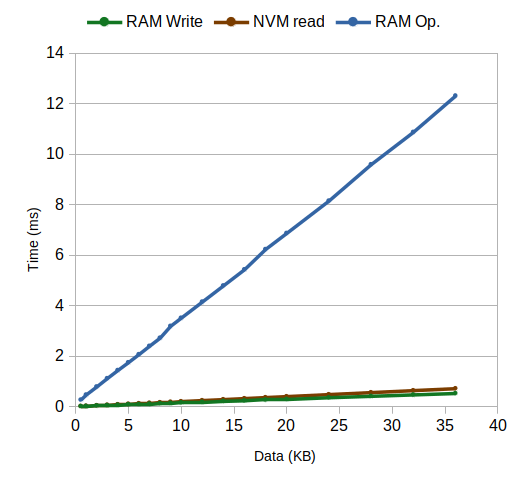
\includegraphics[width=0.7\textwidth]{./Images/memory-time.png}
	\caption{Performance comparison of RAM and eNVM read operations up to 36 KB}
	\label{fig:performance:memory-time}
\end{figure}

\begin{figure}[h!]
	\centering
	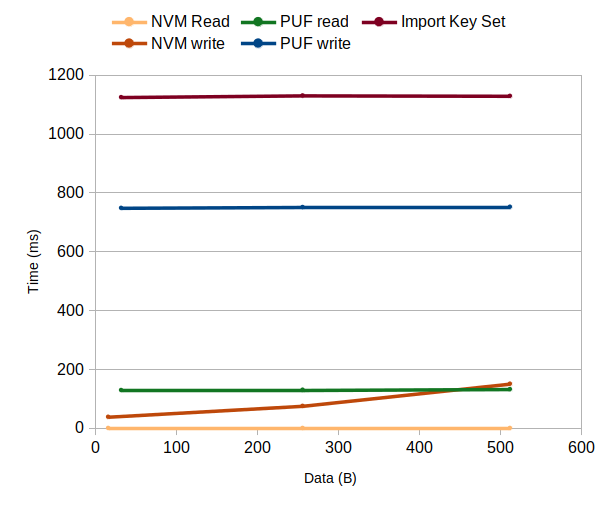
\includegraphics[width=0.7\textwidth]{./Images/nvm-puf-time.png}
	\caption{Performance comparison of PUF and eNVM read and writes, along with the key importation service}
	\label{fig:performance:nvm-puf-time}
\end{figure}

\begin{figure}[h!]
	\centering
	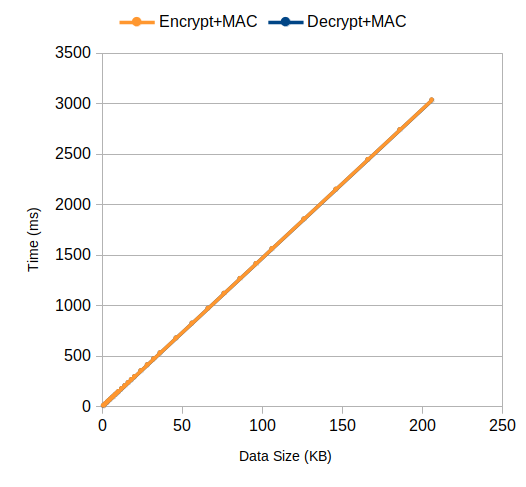
\includegraphics[width=0.7\textwidth]{./Images/services-time.png}
	\caption{Performance comparison of continuous encryption and MAC and continuous decryption and MAC}
	\label{fig:performance:services-time}
\end{figure}

%% If Printing on DOUBLE SIDED pages, the second page should be white.
%% Otherwise, comment the following command:
% \cleardoublepage

% -----------------------------------------------------------------------------
% And this is THE END of the IST Thesis Document
\end{document}
